\documentclass[10pt]{article}
\usepackage[a4paper,margin=0.72in]{geometry}
\usepackage{graphicx,booktabs,amsmath,amssymb,float,longtable,array,microtype}
\usepackage[font=small,labelfont=bf]{caption}
\usepackage{subcaption}
\usepackage{xcolor}
\usepackage[hidelinks]{hyperref}
\usepackage{enumitem}
\setlist{nosep,leftmargin=*}
\graphicspath{{../outputs/figures/}}
\newcommand{\RPS}{\operatorname{RPS}}
\newcommand{\E}{\mathbb{E}}
\title{Forecasting Competitive Football\\
\large Leakage-Safe Pre-Match and In-Play Prediction from Raw Event Data}
\author{Machine Learning Final Project}
\date{August 2026}

\begin{document}
\maketitle

\begin{abstract}
This work builds three football forecasting systems from raw StatsBomb events and Football-Data odds: pre-match H/D/A classification, pre-match clipped goal-margin regression, and five-minute in-play classification/regression. It reproduces the P1 multilayer-network construction and independently implements the P2 Fast Interpretable Greedy-Tree Sums (FIGS) algorithm. The received 79-match ``test'' had already been inspected, so it is retained only as a pilot. A chronologically later StatsBomb 2016/17 cohort was cryptographically sealed and evaluated exactly once after all code, features, calibration, and model choices were locked. StatsBomb exposes only 34 Barcelona-centred matches for that season, so final intervals are wide and the cohort is not league-representative. On this cohort, Platt-calibrated random forest achieved pre-match RPS 0.120 versus 0.131 for the raw market, but the paired difference interval included zero. Raw in-play gradient boosting achieved overall RPS 0.116 and RPS 0.082 at minute 90. The central negative result is equally important: market-only features were strongest in development, network additions were inconsistent, and calibration often improved ECE without improving proper scores.
\end{abstract}

\section{Introduction \& Problem Framing}

Let match $i$ have final home and away goals $(g_i^H,g_i^A)$ and ordered outcome $Y_i\in\{A,D,H\}$. The project defines three tasks before fitting any model.

\textbf{Model 1 (C), pre-match classification.} From a kickoff-time feature vector $x_i^{(0)}$, estimate calibrated probabilities $\hat p_i(A),\hat p_i(D),\hat p_i(H)$. Ranked probability score (RPS) is the headline metric; log loss, multiclass Brier score, expected calibration error (ECE), and accuracy are always reported alongside it.

\textbf{Model 2 (R), pre-match regression.} Predict
\[
M_i=\operatorname{clip}(g_i^H-g_i^A,-5,5)
\]
from the same pre-match information. MAE is the headline metric, with RMSE and Pearson correlation as complements. A multinomial logistic mapper fitted only on the calibration block converts each scalar margin forecast into H/D/A probabilities.

\textbf{Model 3 (L), in-play forecasting.} At snapshot time $t\in\{0,5,\ldots,90\}$ minutes, estimate both $P(Y_i\mid x_i^{(t)})$ and $M_i$ using frozen pre-match variables plus events satisfying $s\leq 60t$ exactly. All snapshots from a match share a split. The frozen market and frozen best pre-match forecast are sanity baselines.

The study asks whether historical event and P1 network summaries improve over market and conventional form, how rapidly live state improves forecasts, and whether a compact P2 model offers a useful accuracy--interpretability trade-off. No hypothesis assumes that a student model should beat a mature betting market.

\section{Dataset, Integration Design \& Competition Selection}

StatsBomb open data supplies event streams, fixtures, teams, players, and lineups \cite{statsbomb}. Football-Data supplies B365 H/D/A odds \cite{footballdata}. The normalized relational store contains 414 matches, 1,420,167 events, 14,899 match-player lineup rows, 657 players, and 23 teams. La Liga 2015/16 is complete (380 matches) and forms the development backbone. The adjacent 2016/17 StatsBomb release contains only 34 available matches, largely involving Barcelona; it is used as the chronologically later final cohort because the original 2015/16 tail was already opened.

Odds are joined by exact cleaned date, home alias, and away alias. Scores, results, and match statistics are never join keys. All 414 StatsBomb fixtures match exactly; duplicate keys and exclusions are zero. Decimal odds $o_k$ become implied probabilities $q_k=1/o_k$, overround $b=\sum_k q_k$, and de-vigged market probabilities $p_k=q_k/b$. The alias table and every join diagnostic are exported. Selected seasons have no StatsBomb 360 files; an empty typed table and source availability manifest preserve that fact instead of inventing data.

StatsBomb uses a common team-in-possession attacking orientation. Empirically, home and away shots start at mean $x=104.09$ and $103.53$, while mean pass displacements are $+7.79$ and $+8.55$. Therefore no home/away pitch flip is applied (Figure~\ref{fig:orientation}).

\begin{figure}[H]
\centering
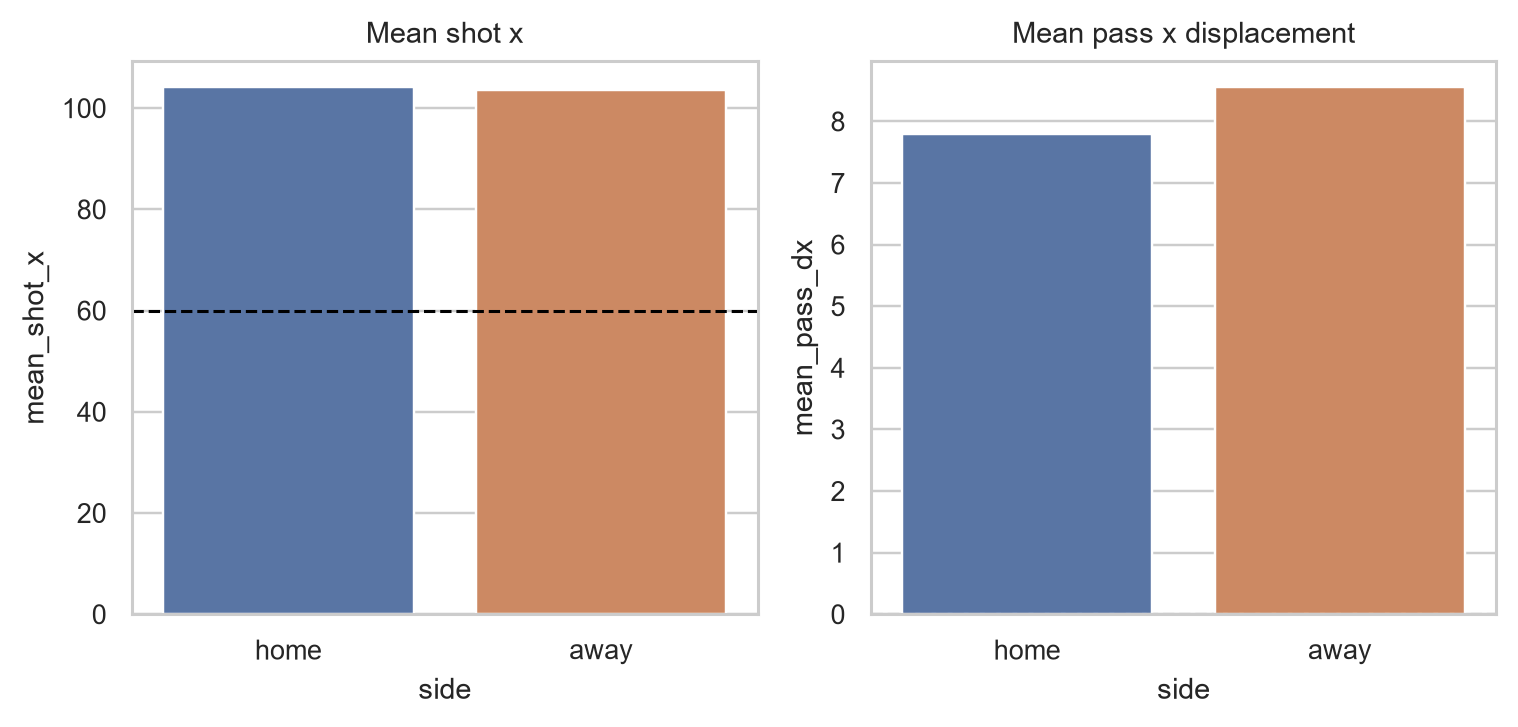
\includegraphics[width=.68\textwidth]{p1/p1_orientation_validation.png}
\caption{Orientation validation. Both sides attack toward increasing x in the StatsBomb event frame.}
\label{fig:orientation}
\end{figure}

\section{Feature Engineering: Pre-Match and In-Play Pipelines}

\subsection*{Pre-match pipeline}

Each match has 391 numeric predictors. Conventional histories include goals, points, shots, shots on target, xG, passes, pass completion, final-third entries, pressures, recoveries, interceptions, fouls, yellow/red cards, carries, duels, possessions, rest, calendar context, and market overround. For each team, raw match statistics are shifted first and then summarized by 3/5/10-match rolling means and expanding means. Home, away, and difference views are retained. P1 histories use the same shift-before-roll design for centrality, leakage, recovery, switching, pass, and possession-transition summaries. Four explicit source timestamps are strictly earlier than kickoff for every row.

Feature groups are frozen as market (3), conventional (226), network (162), conventional+market (229), conventional+network (388), and combined (391). Targets and scores do not appear in the feature file.

\subsection*{In-play pipeline}

Nineteen snapshots per match yield 7,866 rows. The event clock includes timestamp milliseconds; the predicate is \texttt{event\_seconds\_exact <= snapshot\_seconds}. A test proves that 30:00.000 is included and 30:00.001 is excluded. Cumulative, recent-five-minute, and recent-ten-minute home/away/difference features cover score, shots/xG, passes/completion, final-third entries, pressures, recoveries, interceptions, fouls/cards, carries, and current possession. All 391 pre-match features are copied unchanged into every match snapshot. There are zero boundary violations and every match has exactly one role.

The 2016/17 event subset omits most non-Barcelona league fixtures. Thus rolling histories during that season are incomplete relative to the real league schedule; this is a source-coverage limitation, not a leakage fixable by modeling.

\section{Paper Reproductions (P1 \& P2)}

\subsection*{P1: multilayer network framework}

Following Novillo et al. \cite{novillo2024}, the $120\times80$ pitch is divided into $4\times5=20$ zones. For each team, completed passes add directed intra-layer edges. Consecutive, same-period possession changes add inter-layer edges from the final spatial event of the old possession to the first spatial event of the new possession. Late events tagged to an earlier possession are removed at the next possession boundary. With home/away pass matrices $A_H,A_A$ and transition matrices $C_{HA},C_{AH}$,
\[
\mathcal A=\begin{bmatrix} A_H&C_{HA}\\C_{AH}&A_A\end{bmatrix}\in\mathbb R_+^{40\times40}.
\]
The paper-specified dominant \emph{right} eigenvector solves $\mathcal A x=\lambda_{\max}x$ and is normalized to unit sum. For zone $j$, with pass in-degree $d^{P,in}_j$ and inter-layer degrees $d^{I,in}_j,d^{I,out}_j$,
\[
L_j=\frac{d^{I,out}_j}{d^{P,in}_j+d^{I,in}_j},\quad
R_j=\frac{d^{I,in}_j}{d^{P,in}_j+d^{I,in}_j},\quad
S=\frac12\sum_{j:d^{P,in}_j>0}\frac{d^{I,in}_j+d^{I,out}_j}{d^{P,in}_j}.
\]
Undefined zone ratios remain missing and denominators are reported.

\begin{figure}[H]
\centering
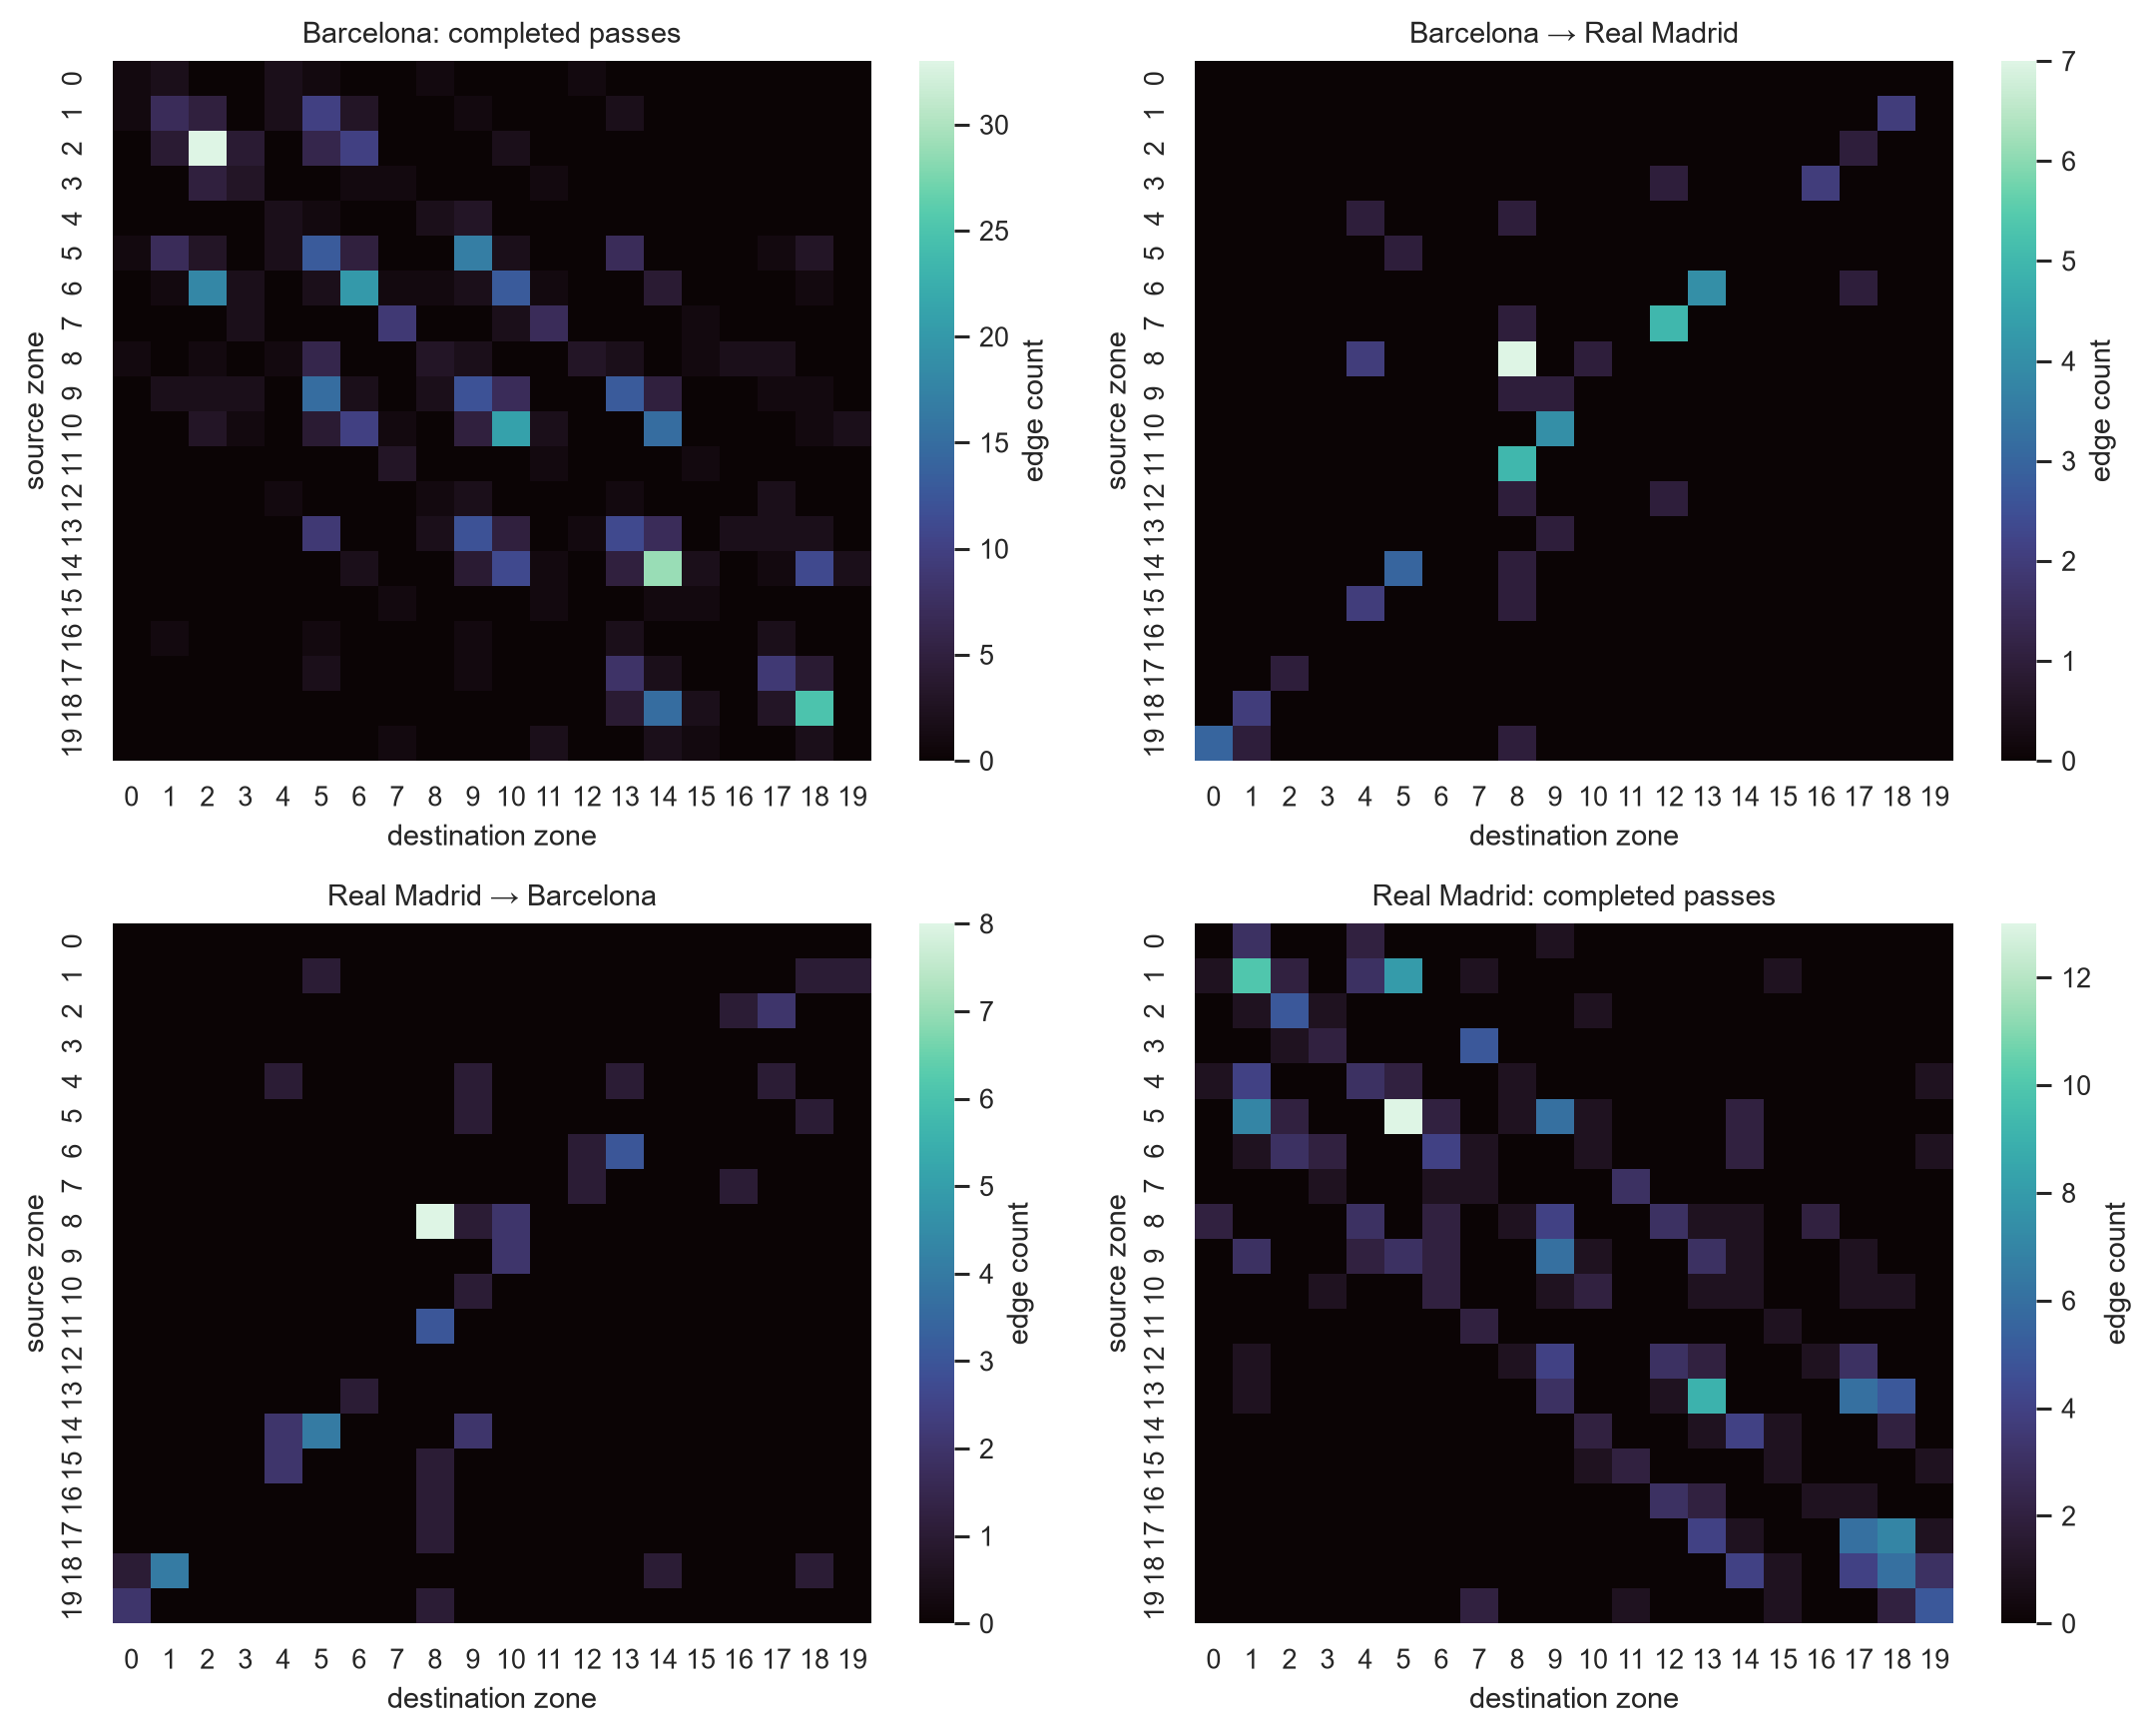
\includegraphics[width=.9\textwidth]{p1/p1_example_multilayer_network.png}
\caption{Example Barcelona--Real Madrid two-layer adjacency blocks. Rows are source zones and columns destinations.}
\label{fig:p1example}
\end{figure}

All 760 development team-match rows match the historical notebook: the largest absolute metric discrepancy is $2.72\times10^{-15}$ and maximum eigen residual is $7.86\times10^{-14}$. Figure~\ref{fig:p1teams} compares zone z-scores. Mean supra centrality and season points correlate at $r=0.561$ over 20 teams, a descriptive association only. Because the paper used Opta 2018/19 and this project uses StatsBomb 2015/16, this is methodological rather than numerical replication.

\begin{figure}[H]
\centering
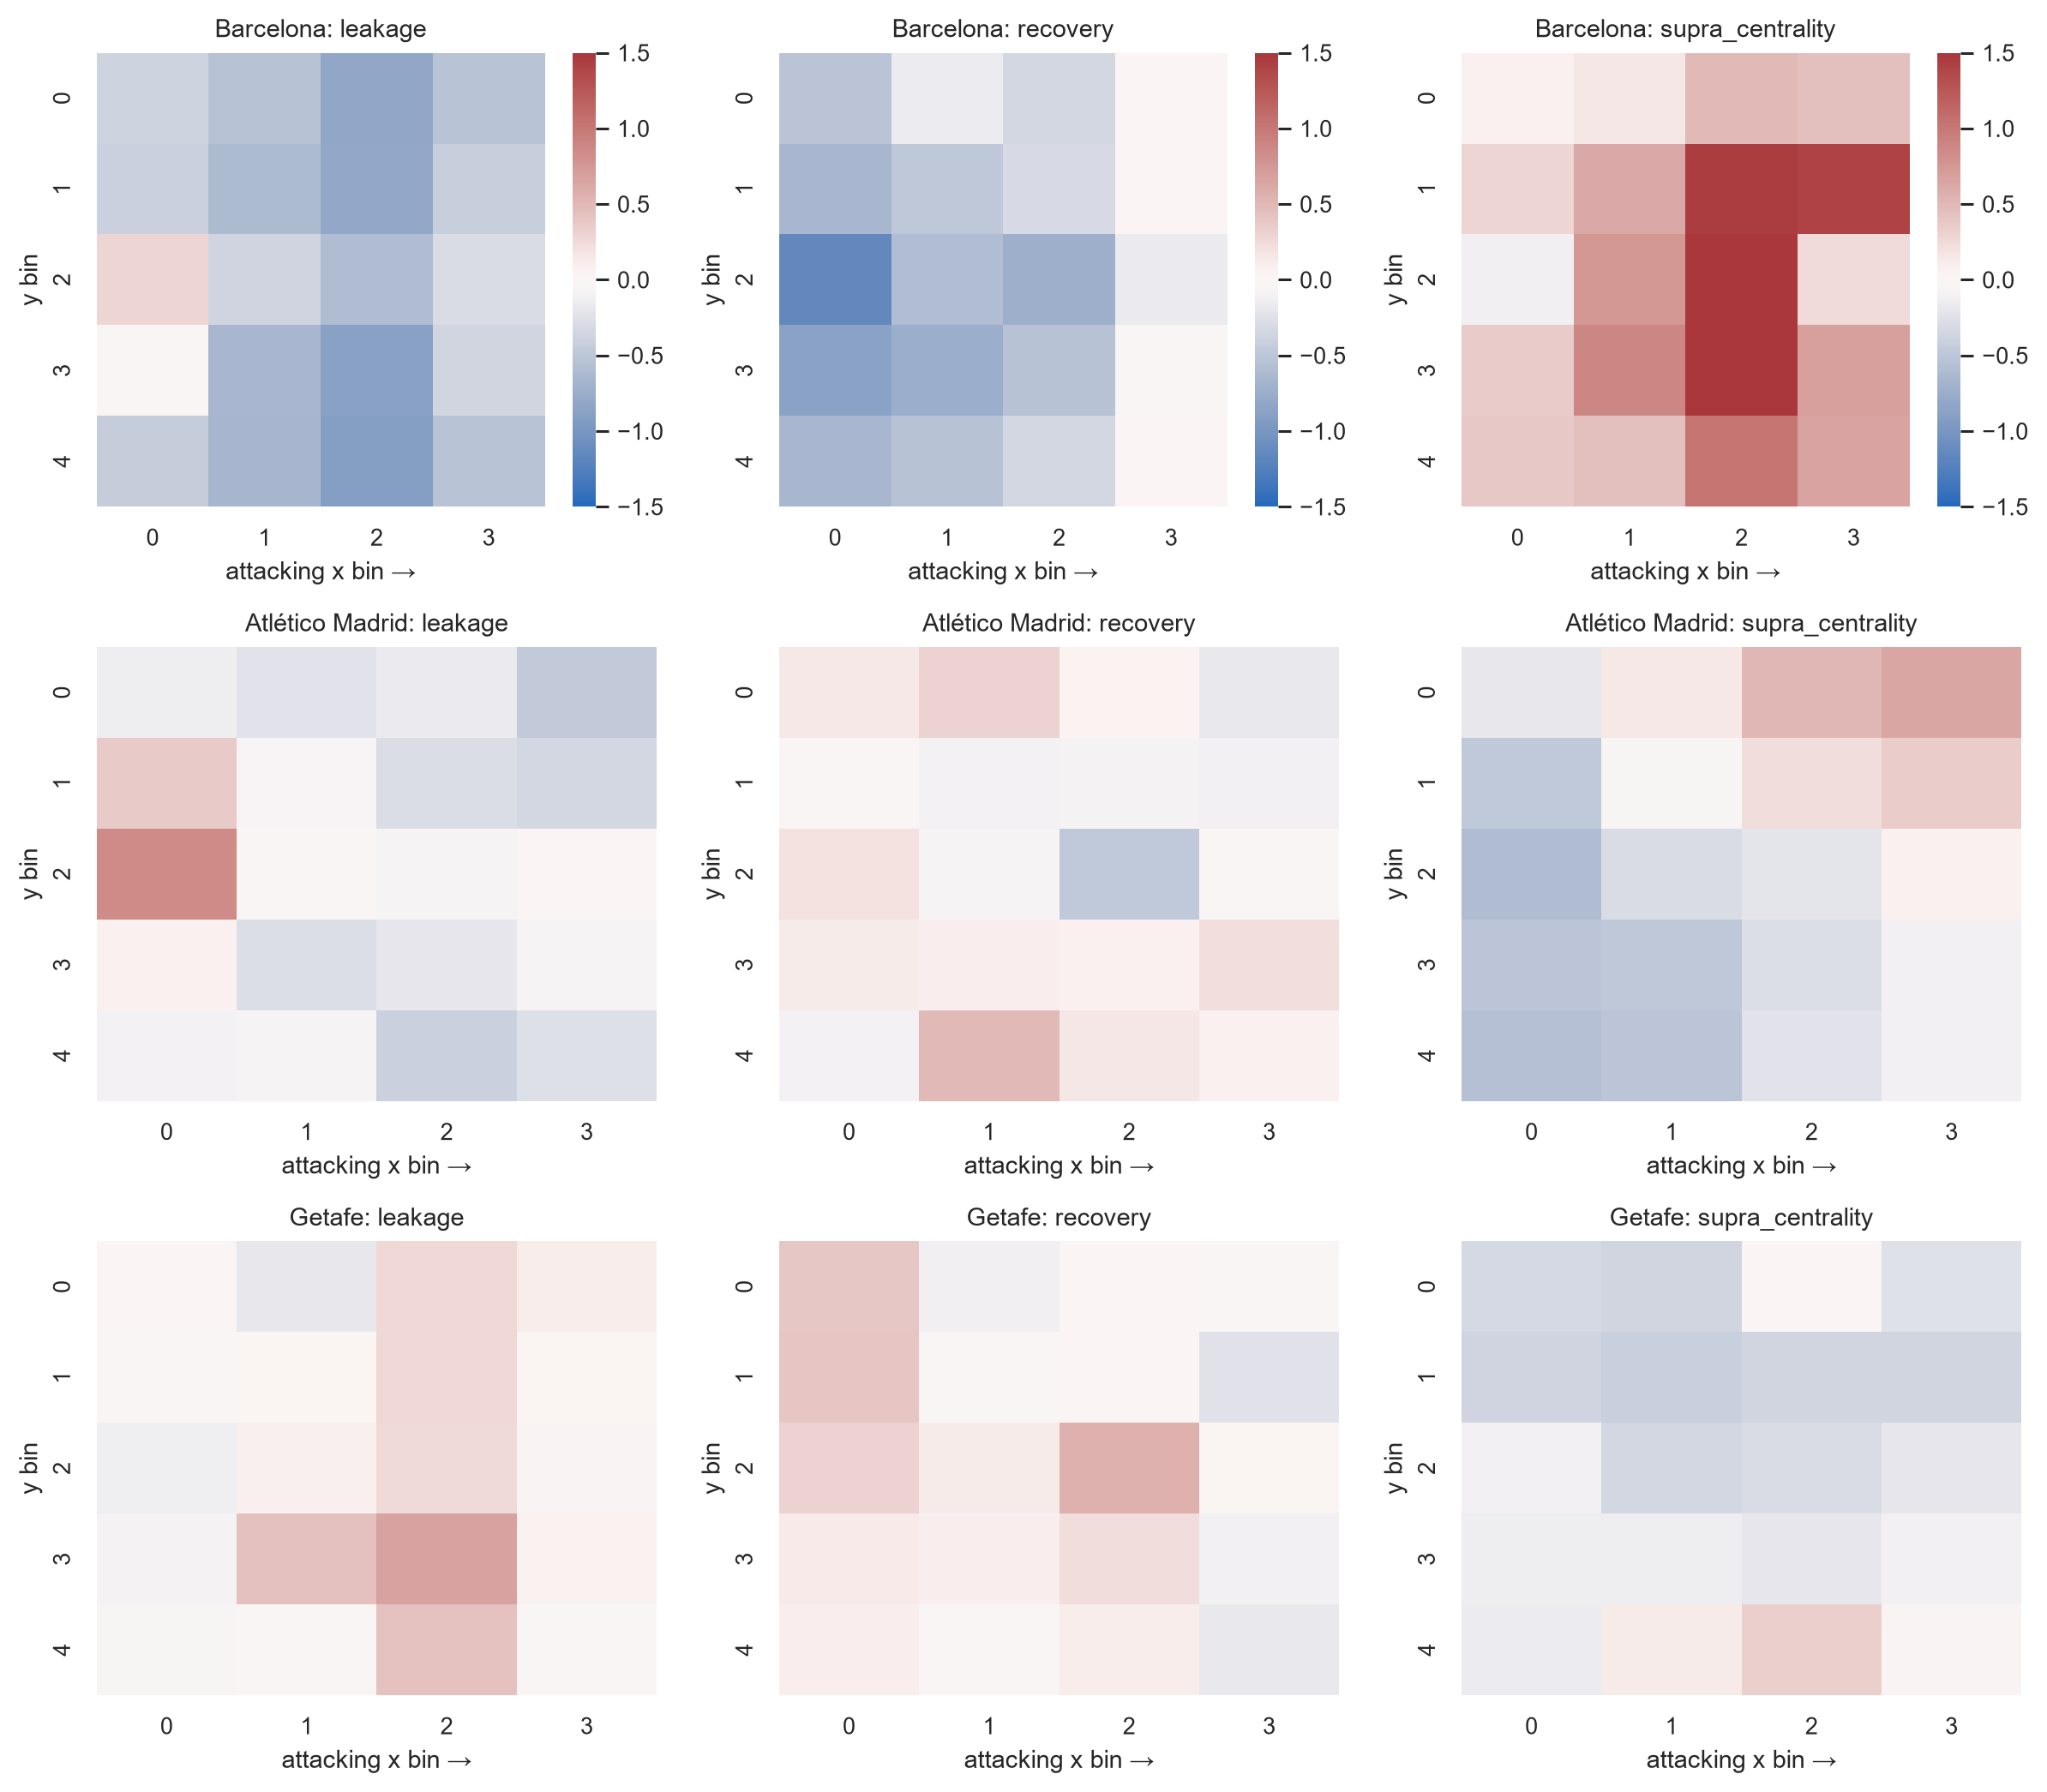
\includegraphics[width=.94\textwidth]{p1/p1_team_zone_comparison.png}
\caption{Team-average zone z-scores. Barcelona concentrates supra-centrality in advanced central zones; patterns are descriptive, not causal.}
\label{fig:p1teams}
\end{figure}

\begin{table}[H]
\centering\scriptsize
\resizebox{\textwidth}{!}{%
\begin{tabular}{lrrrrrr}
\toprule
Team & Pts & Supra cent. & Leakage & Recovery & Switching & Cent. rank \\
\midrule
Barcelona & 91 & 0.870 & 0.132 & 0.110 & 3.188 & 1 \\
Real Madrid & 90 & 0.682 & 0.151 & 0.128 & 4.192 & 2 \\
Atlético Madrid & 88 & 0.464 & 0.196 & 0.167 & 5.501 & 10 \\
Villarreal & 64 & 0.383 & 0.234 & 0.165 & 6.397 & 17 \\
Athletic Club & 62 & 0.473 & 0.204 & 0.168 & 5.539 & 9 \\
Celta Vigo & 60 & 0.658 & 0.187 & 0.145 & 4.780 & 3 \\
Sevilla & 52 & 0.429 & 0.203 & 0.143 & 4.923 & 14 \\
Málaga & 48 & 0.457 & 0.220 & 0.178 & 6.787 & 11 \\
Real Sociedad & 48 & 0.568 & 0.206 & 0.161 & 5.325 & 6 \\
Real Betis & 45 & 0.475 & 0.237 & 0.171 & 6.468 & 8 \\
\bottomrule
\end{tabular}}
\end{table}

\subsection*{P2: scratch FIGS}

FIGS generalizes CART by growing a sum of trees simultaneously \cite{tan2025}. Every current leaf and a possible new root compete for the single largest impurity reduction. For candidate tree $k$, residuals exclude all other trees; accepted splits can later revisit old trees. A global split budget controls interpretability. Optional post-structure backfitting implements the supplement's block coordinate descent.

Production code has no \texttt{imodels} import. Tests cover the paper toy, earlier-tree revisits, deterministic multiclass probabilities, zero-rule constants, backfitting monotonicity, and sklearn API shape. On fixed regression and multiclass toys, predictions match the independent \texttt{imodels} reference to $10^{-12}$. One fidelity nuance is explicit: the paper prose describes Gini classification, while the official residualized multiclass reference fits one-hot targets with multi-output least-squares stumps and applies softmax. The scratch classifier follows the reproducible reference behavior because Gini is not defined for continuous residual vectors after the first component.

\begin{figure}[H]
\centering
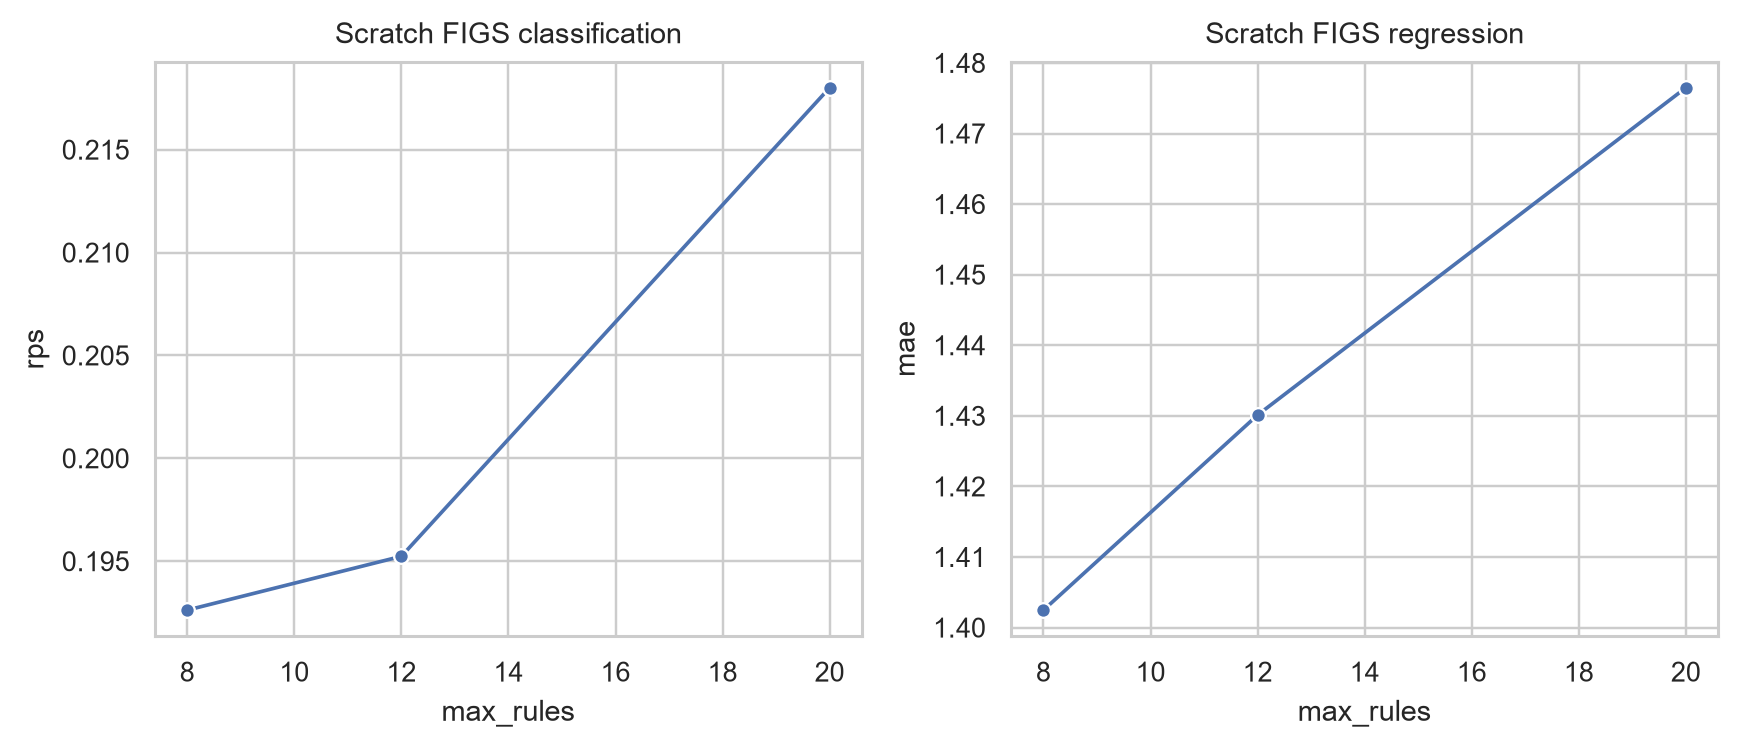
\includegraphics[width=.7\textwidth]{models/figs_split_budget.png}
\caption{Validation performance versus scratch-FIGS split budget. More rules did not monotonically improve football generalization.}
\end{figure}

\section{Experimental Setup}

The 2015/16 roles are 189 train, 50 validation, 62 calibration, and 79 opened pilot matches. The pilot starts 2 April 2016 and is never called final. All 34 available 2016/17 matches are final. Before opening them, SHA-256 hashes froze 21 files containing source, features, splits, specifications, calibration, and the final evaluator. The evaluator produced forecasts before reading labels, wrote a permanent open marker, scored once, and now refuses rerun.

Classification RPS uses class order A--D--H:
\[
\RPS=\frac1{N(K-1)}\sum_i\sum_{k=1}^{K-1}
\left(\sum_{j\le k}\hat p_{ij}-\sum_{j\le k}y_{ij}\right)^2.
\]
Brier is the mean sum over three squared class errors. ECE uses ten equal-width top-label bins. Platt scaling is multinomial logistic scaling of log probabilities; isotonic is one-versus-rest followed by normalization. Both are fitted only on calibration. Model 3 calibrators are separate for early ($\le30$), middle (35--60), and late ($>60$) phases. Platt was fixed for final before labels; raw probabilities remain visible. Bootstrap intervals resample matches; snapshot intervals resample entire matches, never individual rows.

The required families are evaluated: dummy, SVC/SVR, exact and Nystroem kernels, random forest, gradient boosting, XGBoost \cite{xgboost}, LightGBM \cite{lightgbm}, market, P1-only linear models, and scratch FIGS. Development selection minimizes RPS or MAE. Final base models use train+validation+pilot, while calibration remains disjoint.

\section{Results: Models 1, 2, and 3}

\subsection*{Model 1}

Table~\ref{tab:m1note} contains every final pre-match classifier and both raw/Platt outputs. Random-forest/Platt RPS is 0.120 (95\% bootstrap 0.070--0.185), compared with 0.131 for the raw market. The paired mean improvement is $-0.0116$, but its interval $[-0.0495,0.0168]$ includes zero. Accordingly, the result is a small-cohort estimate, not evidence of market superiority. P1-only logistic and SVC degrade sharply under the Barcelona-centred distribution shift.

\phantomsection\label{tab:m1note}
\begin{table}[H]
\centering\scriptsize
\resizebox{\textwidth}{!}{%
\begin{tabular}{lrrrrrrrr}
\toprule
Model & Cal. & RPS & Log loss & Brier & ECE & Acc. & CI low & CI high \\
\midrule
random\_forest & platt & \textbf{0.120} & 0.664 & \textbf{0.359} & 0.112 & 0.765 & 0.070 & 0.185 \\
gradient\_boosting & platt & 0.125 & 0.683 & 0.360 & 0.063 & 0.765 & 0.063 & 0.206 \\
market & platt & 0.126 & \textbf{0.648} & 0.359 & 0.101 & 0.735 & 0.058 & 0.208 \\
xgboost & raw & 0.127 & 0.697 & 0.379 & 0.157 & 0.765 & 0.071 & 0.191 \\
xgboost & platt & 0.130 & 0.686 & 0.377 & 0.146 & 0.765 & 0.081 & 0.187 \\
random\_forest & raw & 0.131 & 0.705 & 0.387 & 0.157 & 0.765 & 0.086 & 0.181 \\
lightgbm & raw & 0.131 & 0.726 & 0.383 & 0.102 & 0.765 & 0.062 & 0.216 \\
market & raw & 0.131 & 0.685 & 0.372 & 0.122 & 0.735 & 0.066 & 0.210 \\
gradient\_boosting & raw & 0.132 & 0.714 & 0.383 & 0.198 & 0.765 & 0.077 & 0.199 \\
lightgbm & platt & 0.160 & 0.832 & 0.458 & 0.248 & \textbf{0.794} & 0.104 & 0.228 \\
scratch\_figs & raw & 0.185 & 0.884 & 0.513 & 0.227 & 0.706 & 0.162 & 0.213 \\
scratch\_figs & platt & 0.187 & 0.888 & 0.513 & 0.210 & 0.706 & 0.165 & 0.215 \\
p1\_logistic & raw & 0.232 & 7.198 & 0.824 & 0.411 & 0.588 & 0.140 & 0.324 \\
svc\_rbf & raw & 0.241 & 1.018 & 0.614 & 0.045 & 0.500 & 0.217 & 0.266 \\
dummy & raw & 0.243 & 1.032 & 0.621 & \textbf{0.003} & 0.500 & 0.208 & 0.278 \\
dummy & platt & 0.244 & 1.028 & 0.622 & 0.097 & 0.500 & 0.227 & 0.258 \\
svc\_rbf & platt & 0.257 & 1.080 & 0.656 & 0.053 & 0.353 & 0.234 & 0.278 \\
p1\_logistic & platt & 0.419 & 7.726 & 0.985 & 0.516 & 0.471 & 0.279 & 0.566 \\
\bottomrule
\end{tabular}}
\end{table}

\begin{figure}[H]
\centering
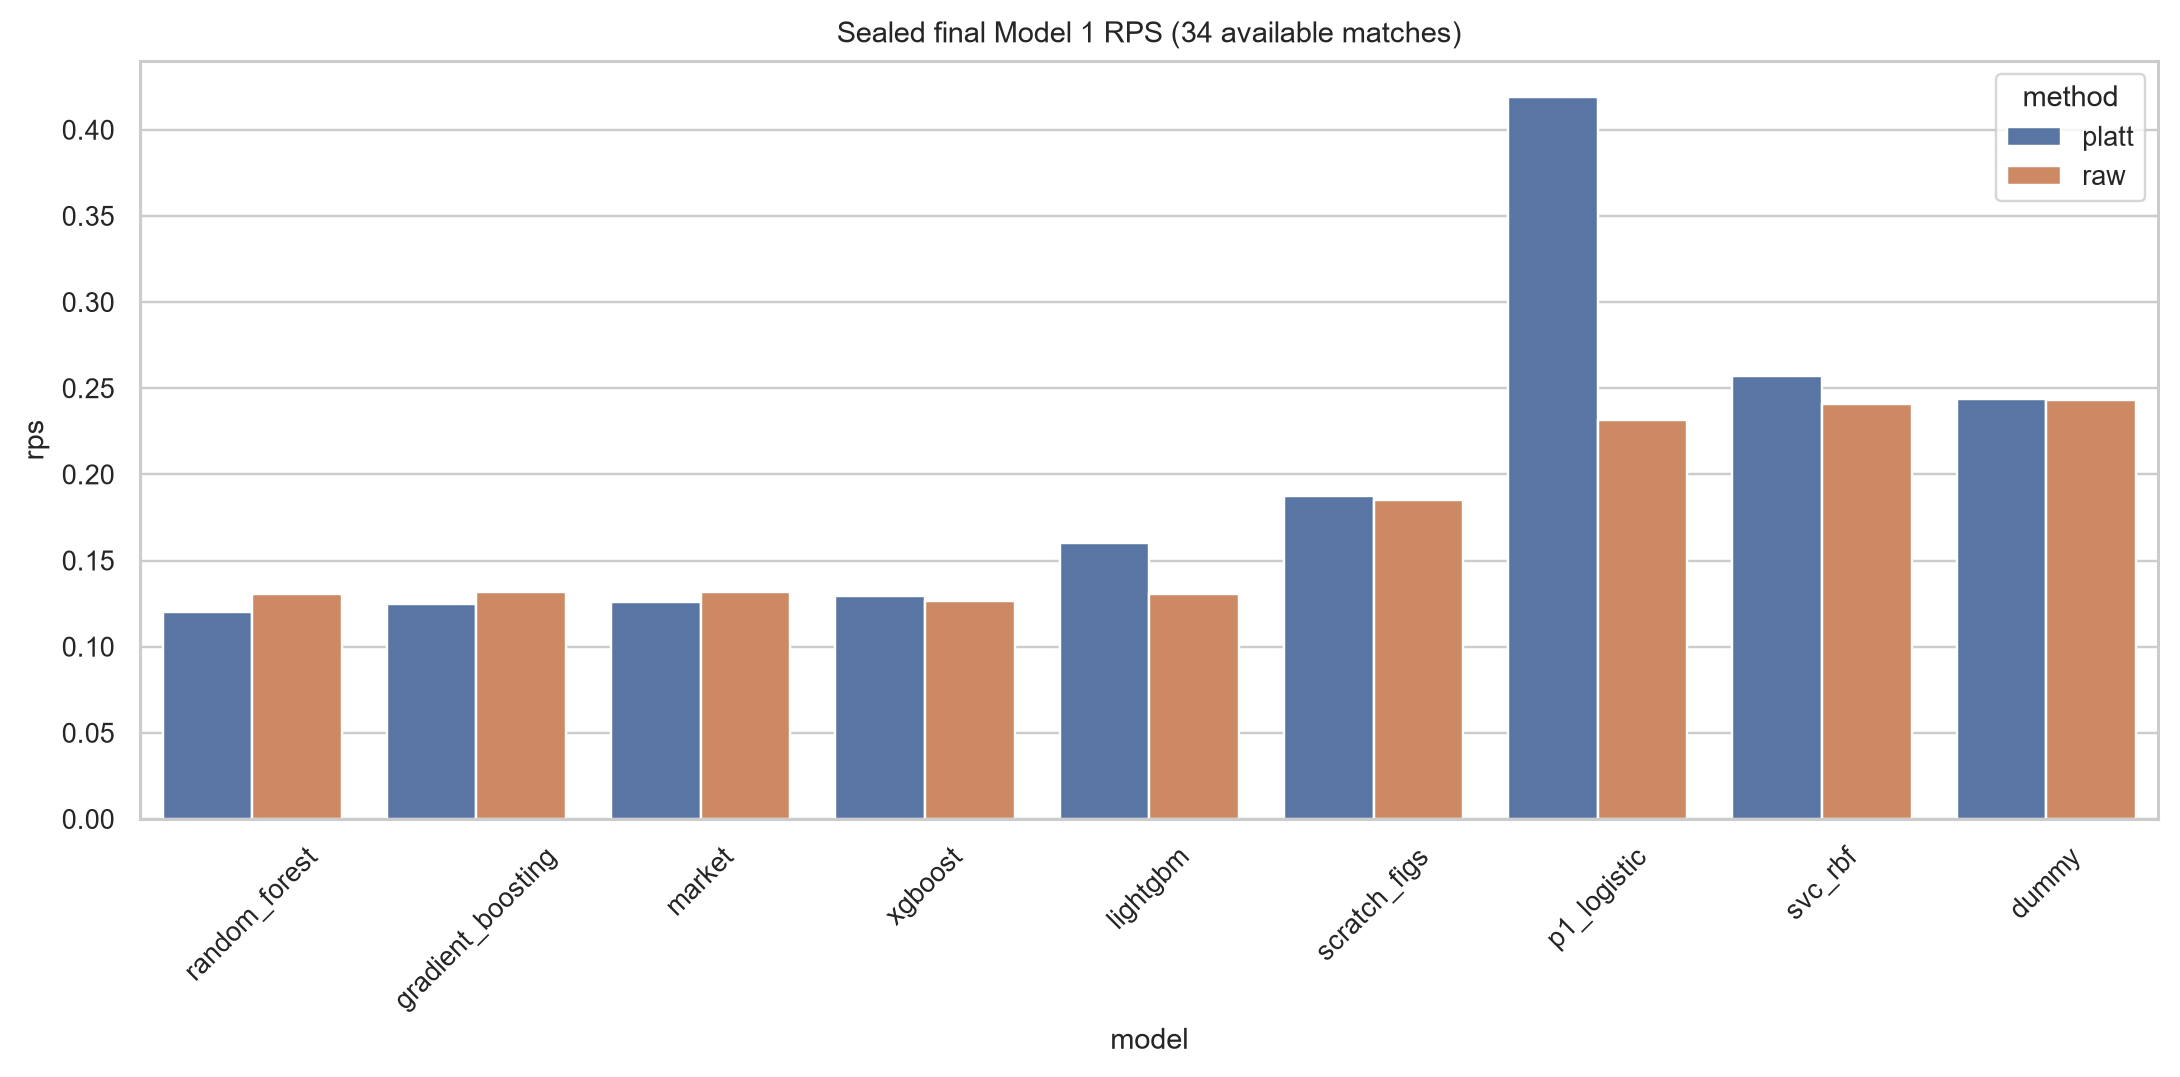
\includegraphics[width=.8\textwidth]{final/final_model1_rps.png}
\caption{Final Model 1 RPS. Confidence intervals overlap strongly because $N=34$.}
\end{figure}

\subsection*{Model 2}

Random forest has the best final MAE (1.479), followed by gradient boosting, LightGBM, XGBoost, and scratch FIGS. Its margin-to-outcome mapper attains RPS 0.116. Exact and approximate kernels collapse toward the dummy under distribution shift, illustrating that their comparable development scores did not guarantee transfer.

\begin{table}[H]
\centering\scriptsize
\resizebox{\textwidth}{!}{%
\begin{tabular}{lrrrrrrr}
\toprule
Model & MAE & RMSE & $r$ & H/D/A RPS & H/D/A LL & CI low & CI high \\
\midrule
random\_forest & \textbf{1.479} & \textbf{1.792} & \textbf{0.766} & \textbf{0.116} & \textbf{0.624} & 1.139 & 1.816 \\
gradient\_boosting & 1.580 & 1.889 & 0.745 & 0.127 & 0.670 & 1.251 & 1.943 \\
lightgbm & 1.582 & 1.848 & 0.744 & 0.124 & 0.661 & 1.272 & 1.887 \\
xgboost & 1.591 & 1.894 & 0.730 & 0.123 & 0.659 & 1.240 & 1.933 \\
scratch\_figs & 1.640 & 2.043 & 0.752 & 0.130 & 0.674 & 1.263 & 2.073 \\
svr\_rbf & 2.291 & 2.765 & 0.211 & 0.244 & 1.035 & 1.763 & 2.791 \\
kernel\_ridge\_exact & 2.294 & 2.839 & 0.211 & 0.262 & 1.093 & 1.735 & 2.853 \\
nystroem\_ridge & 2.294 & 2.765 & 0.211 & 0.243 & 1.026 & 1.785 & 2.805 \\
dummy & 2.294 & 2.767 & -- & 0.244 & 1.028 & 1.769 & 2.821 \\
p1\_ridge & 4.011 & 4.754 & -0.376 & 0.461 & 2.459 & 3.198 & 4.853 \\
\bottomrule
\end{tabular}}
\end{table}

\subsection*{Model 3}

Across 646 final snapshots, raw gradient boosting has the best classification RPS (0.116); frozen pre-match RF/Platt is 0.120 and frozen market 0.131. XGBoost has the best margin MAE (1.276), essentially tied with gradient boosting. Full tables preserve calibration variants and baselines.

\begin{table}[H]
\centering\scriptsize
\resizebox{\textwidth}{!}{%
\begin{tabular}{lrrrrrrrr}
\toprule
Model & Cal. & RPS & Log loss & Brier & ECE & Acc. & CI low & CI high \\
\midrule
gradient\_boosting & raw & \textbf{0.116} & \textbf{0.652} & \textbf{0.346} & 0.112 & 0.774 & 0.068 & 0.167 \\
frozen\_best\_prematch & platt & 0.120 & 0.664 & 0.359 & 0.112 & 0.765 & 0.068 & 0.180 \\
xgboost & raw & 0.123 & 0.659 & 0.365 & 0.036 & 0.743 & 0.076 & 0.176 \\
frozen\_market & raw & 0.131 & 0.685 & 0.372 & 0.122 & 0.735 & 0.068 & 0.205 \\
gradient\_boosting & platt & 0.134 & 0.713 & 0.381 & 0.055 & 0.762 & 0.075 & 0.202 \\
scratch\_figs & platt & 0.135 & 0.717 & 0.407 & 0.139 & 0.777 & 0.107 & 0.166 \\
random\_forest & raw & 0.138 & 0.741 & 0.411 & 0.119 & 0.735 & 0.092 & 0.187 \\
xgboost & platt & 0.143 & 0.755 & 0.402 & 0.073 & 0.715 & 0.087 & 0.208 \\
random\_forest & platt & 0.146 & 0.818 & 0.435 & 0.189 & \textbf{0.782} & 0.086 & 0.223 \\
lightgbm & raw & 0.146 & 0.811 & 0.441 & 0.191 & 0.686 & 0.088 & 0.209 \\
lightgbm & platt & 0.147 & 0.767 & 0.421 & 0.042 & 0.735 & 0.093 & 0.204 \\
scratch\_figs & raw & 0.177 & 0.870 & 0.503 & 0.235 & 0.738 & 0.157 & 0.197 \\
dummy & raw & 0.243 & 1.032 & 0.621 & \textbf{0.003} & 0.500 & 0.208 & 0.279 \\
dummy & platt & 0.244 & 1.029 & 0.622 & 0.097 & 0.500 & 0.228 & 0.258 \\
\bottomrule
\end{tabular}}
\end{table}
\begin{table}[H]
\centering\scriptsize
\resizebox{\textwidth}{!}{%
\begin{tabular}{lrrrrrr}
\toprule
Model & MAE & RMSE & $r$ & H/D/A RPS & H/D/A LL & H/D/A Acc. \\
\midrule
xgboost & \textbf{1.276} & \textbf{1.561} & 0.830 & 0.100 & 0.548 & 0.765 \\
gradient\_boosting & 1.276 & 1.583 & \textbf{0.836} & \textbf{0.099} & \textbf{0.529} & 0.757 \\
lightgbm & 1.310 & 1.583 & 0.824 & 0.103 & 0.573 & 0.776 \\
random\_forest & 1.422 & 1.811 & 0.794 & 0.103 & 0.620 & \textbf{0.779} \\
scratch\_figs & 1.619 & 1.981 & 0.741 & 0.125 & 0.692 & 0.721 \\
dummy & 2.294 & 2.767 & -- & 0.244 & 1.029 & 0.500 \\
\bottomrule
\end{tabular}}
\end{table}

\begin{figure}[H]
\centering
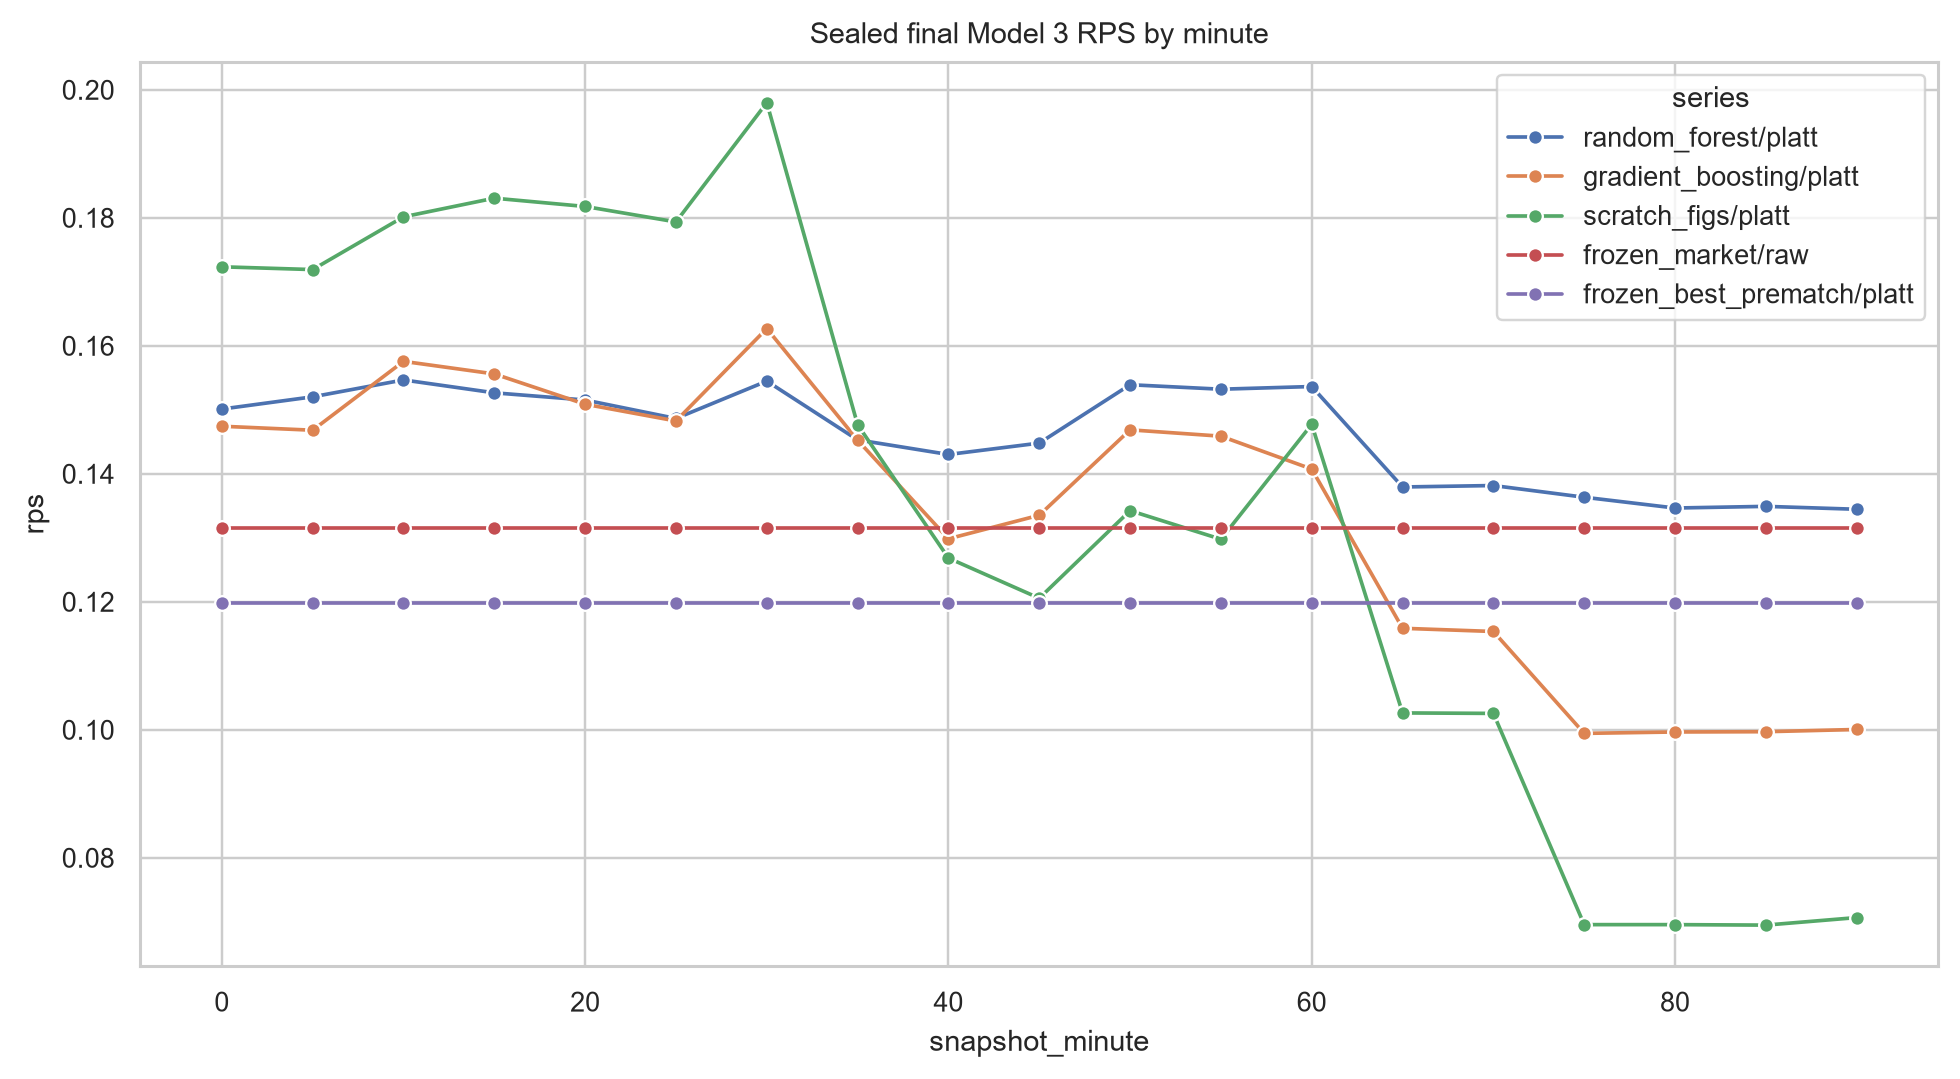
\includegraphics[width=.82\textwidth]{final/final_model3_rps_by_minute.png}
\caption{Final Model 3 RPS by minute against frozen baselines. Phase-Platt FIGS improves strongly late; raw gradient boosting is best overall.}
\label{fig:finalminute}
\end{figure}

\section{Calibration \& Reliability Analysis}

On the final cohort, Platt scaling improves random-forest RPS from 0.131 to 0.120 and ECE from 0.157 to 0.112. Market Platt improves RPS modestly to 0.126. LightGBM and SVC calibration worsen proper scores. These differences reinforce that calibration is a held-out estimation problem rather than an automatic post-processing benefit.

For Model 3, raw gradient boosting has RPS 0.116 and ECE 0.112; phase Platt reduces ECE to 0.055 but worsens RPS to 0.134. Phase sample size is only 62 calibration matches, and repeated snapshots do not create independent labels. Isotonic is more unstable on the opened pilot and was reported there but not selected for final. Figure~\ref{fig:reliability} shows pilot reliability; machine-readable bins for every model/method are retained.

\begin{figure}[H]
\centering
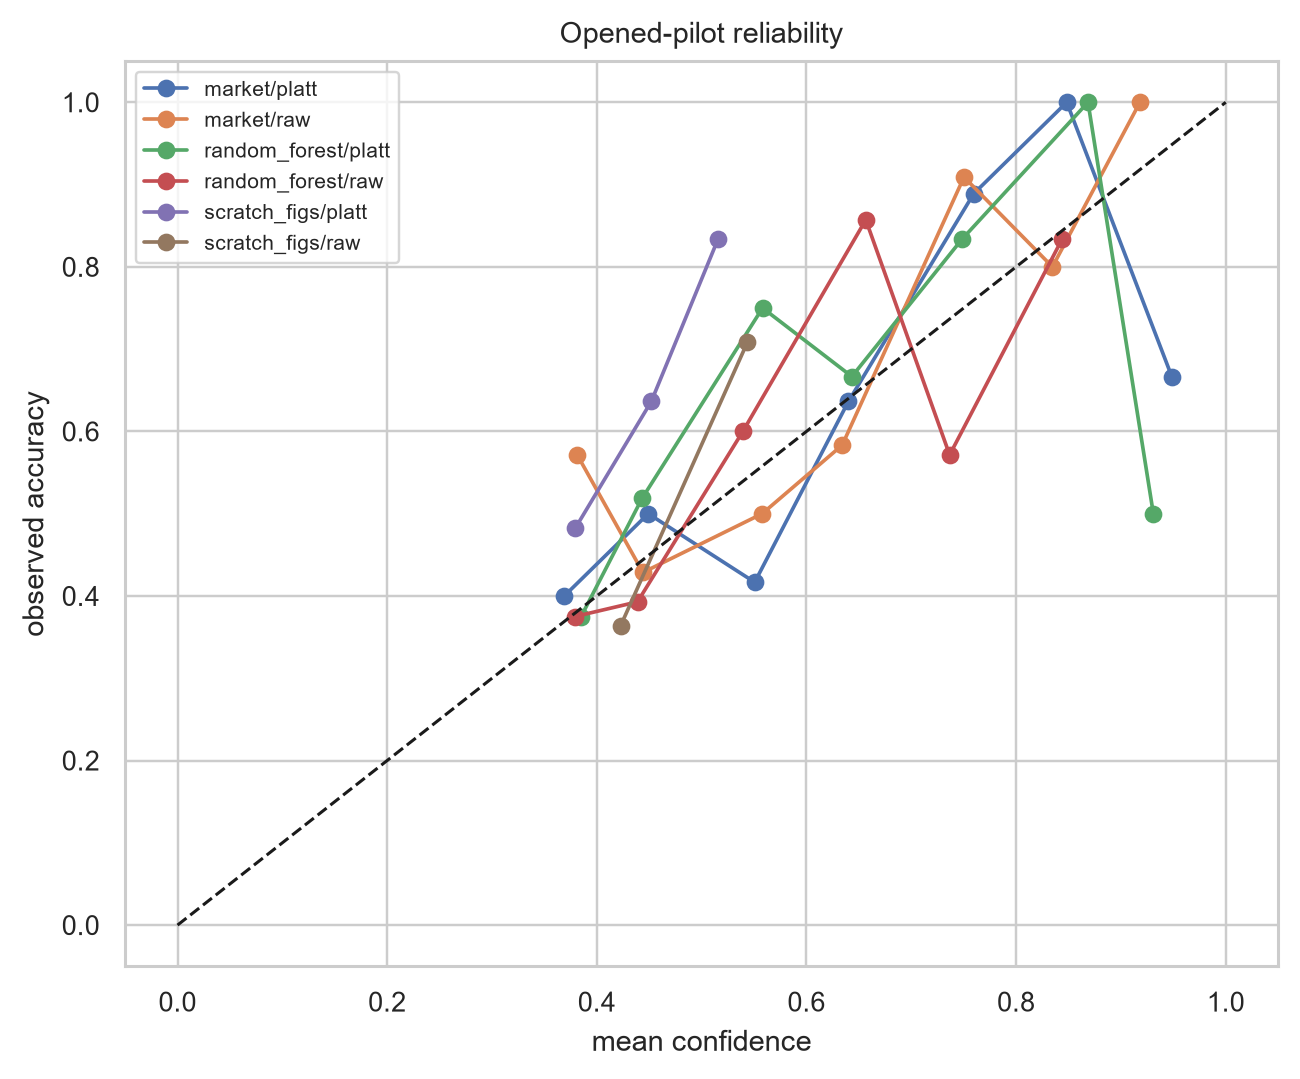
\includegraphics[width=.6\textwidth]{models/model1_reliability.png}
\caption{Opened-pilot top-label reliability. Sparse bins and model-dependent effects motivate the fixed holdout protocol.}
\label{fig:reliability}
\end{figure}

\section{Extended Analysis (8A--8E)}

\subsection*{8A. Error \& Failure Analysis}

The ten worst rows per task are exported with local SHAP values. In the final 34 matches there are only five draws, 16 margins of at least three goals, and nine market upsets. RF/Platt performs worse on draws (mean individual RPS 0.231) than decisive matches (0.101). Its two largest failures are Barcelona away losses at M\'alaga and Deportivo, both predicted as away wins. It substantially corrects one market failure---Barcelona's home loss to Alav\'es---but still predicts H. These cases show the cohort's deliberate Barcelona skew and why accuracy alone (0.765) is misleading.

\begin{figure}[H]
\centering
\begin{subfigure}{.48\textwidth}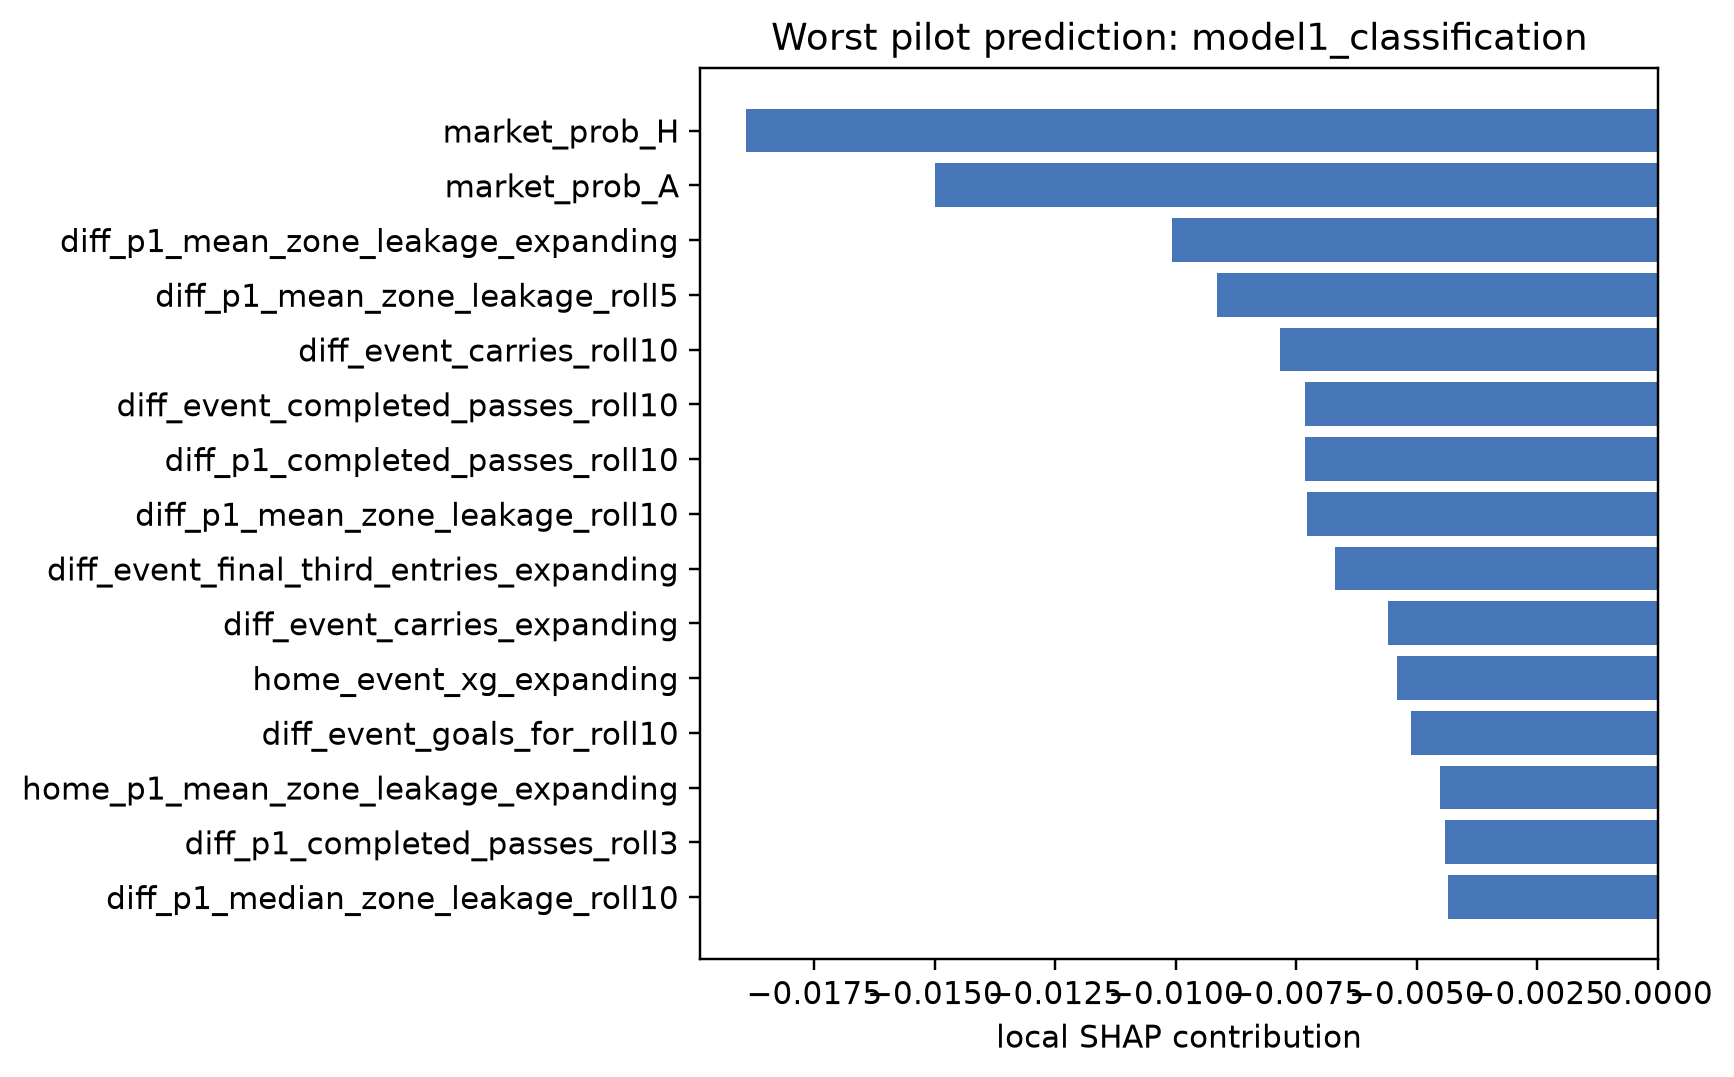
\includegraphics[width=\textwidth]{explainability/model1_classification_worst_local_shap.png}\caption{Worst Model 1 row}\end{subfigure}
\begin{subfigure}{.48\textwidth}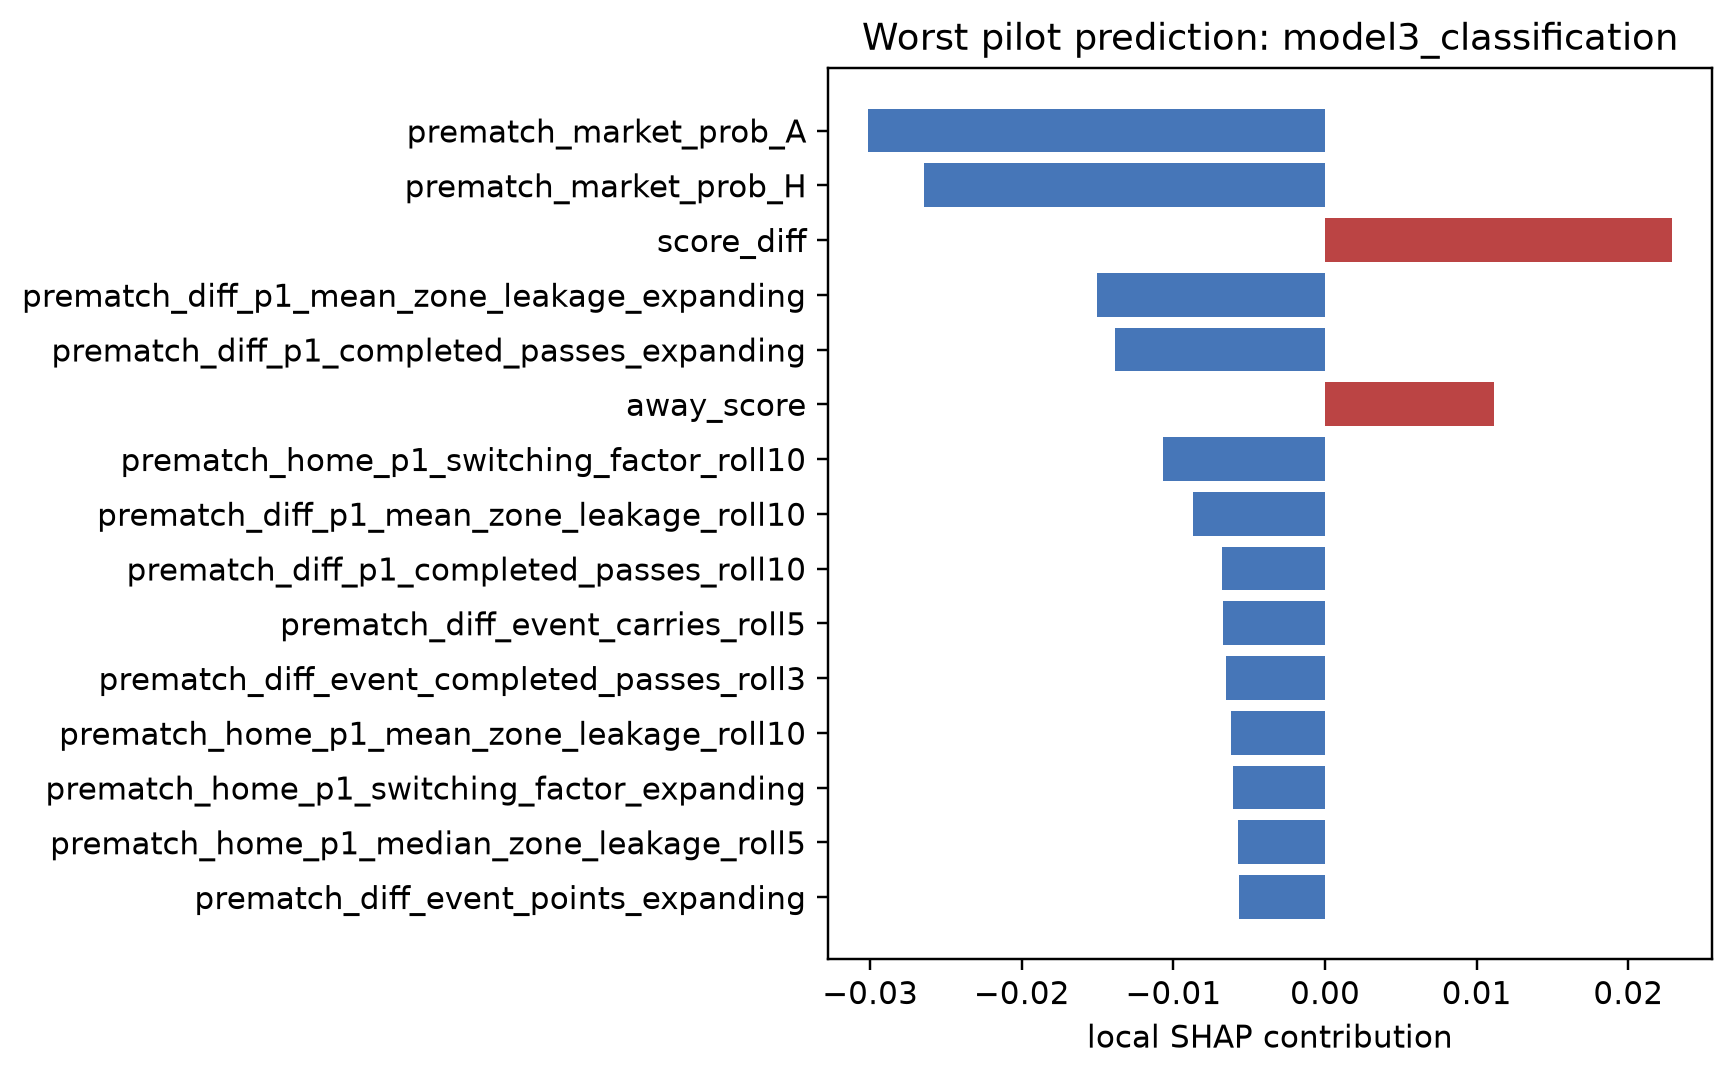
\includegraphics[width=\textwidth]{explainability/model3_classification_worst_local_shap.png}\caption{Worst Model 3 snapshot}\end{subfigure}
\caption{Local random-forest SHAP evidence for worst pilot errors. Red increases and blue decreases the actual-class score.}
\end{figure}

Global SHAP is computed for supported RF, XGBoost, LightGBM, and regression gradient-boosting models. SHAP's TreeExplainer does not support multiclass sklearn \texttt{GradientBoostingClassifier}; the status table records this rather than substituting an unrelated explainer. Market probabilities, score difference, and accumulated conventional/P1 histories dominate supported models.

\subsection*{8B. In-Play Analysis}

At minute 0, raw gradient-boosting RPS is 0.136, slightly worse than the frozen market 0.131. It reaches 0.104 at halftime, 0.087 at minute 75, and 0.082 at minute 90. Phase-Platt scratch FIGS is poor early (0.172 at kickoff) but reaches 0.071 at minute 90. XGBoost margin MAE declines from 1.556 at kickoff to 1.064 at minute 90. Thus event state becomes useful after enough match evidence accumulates, while a pre-match prior remains essential early.

\begin{figure}[H]
\centering
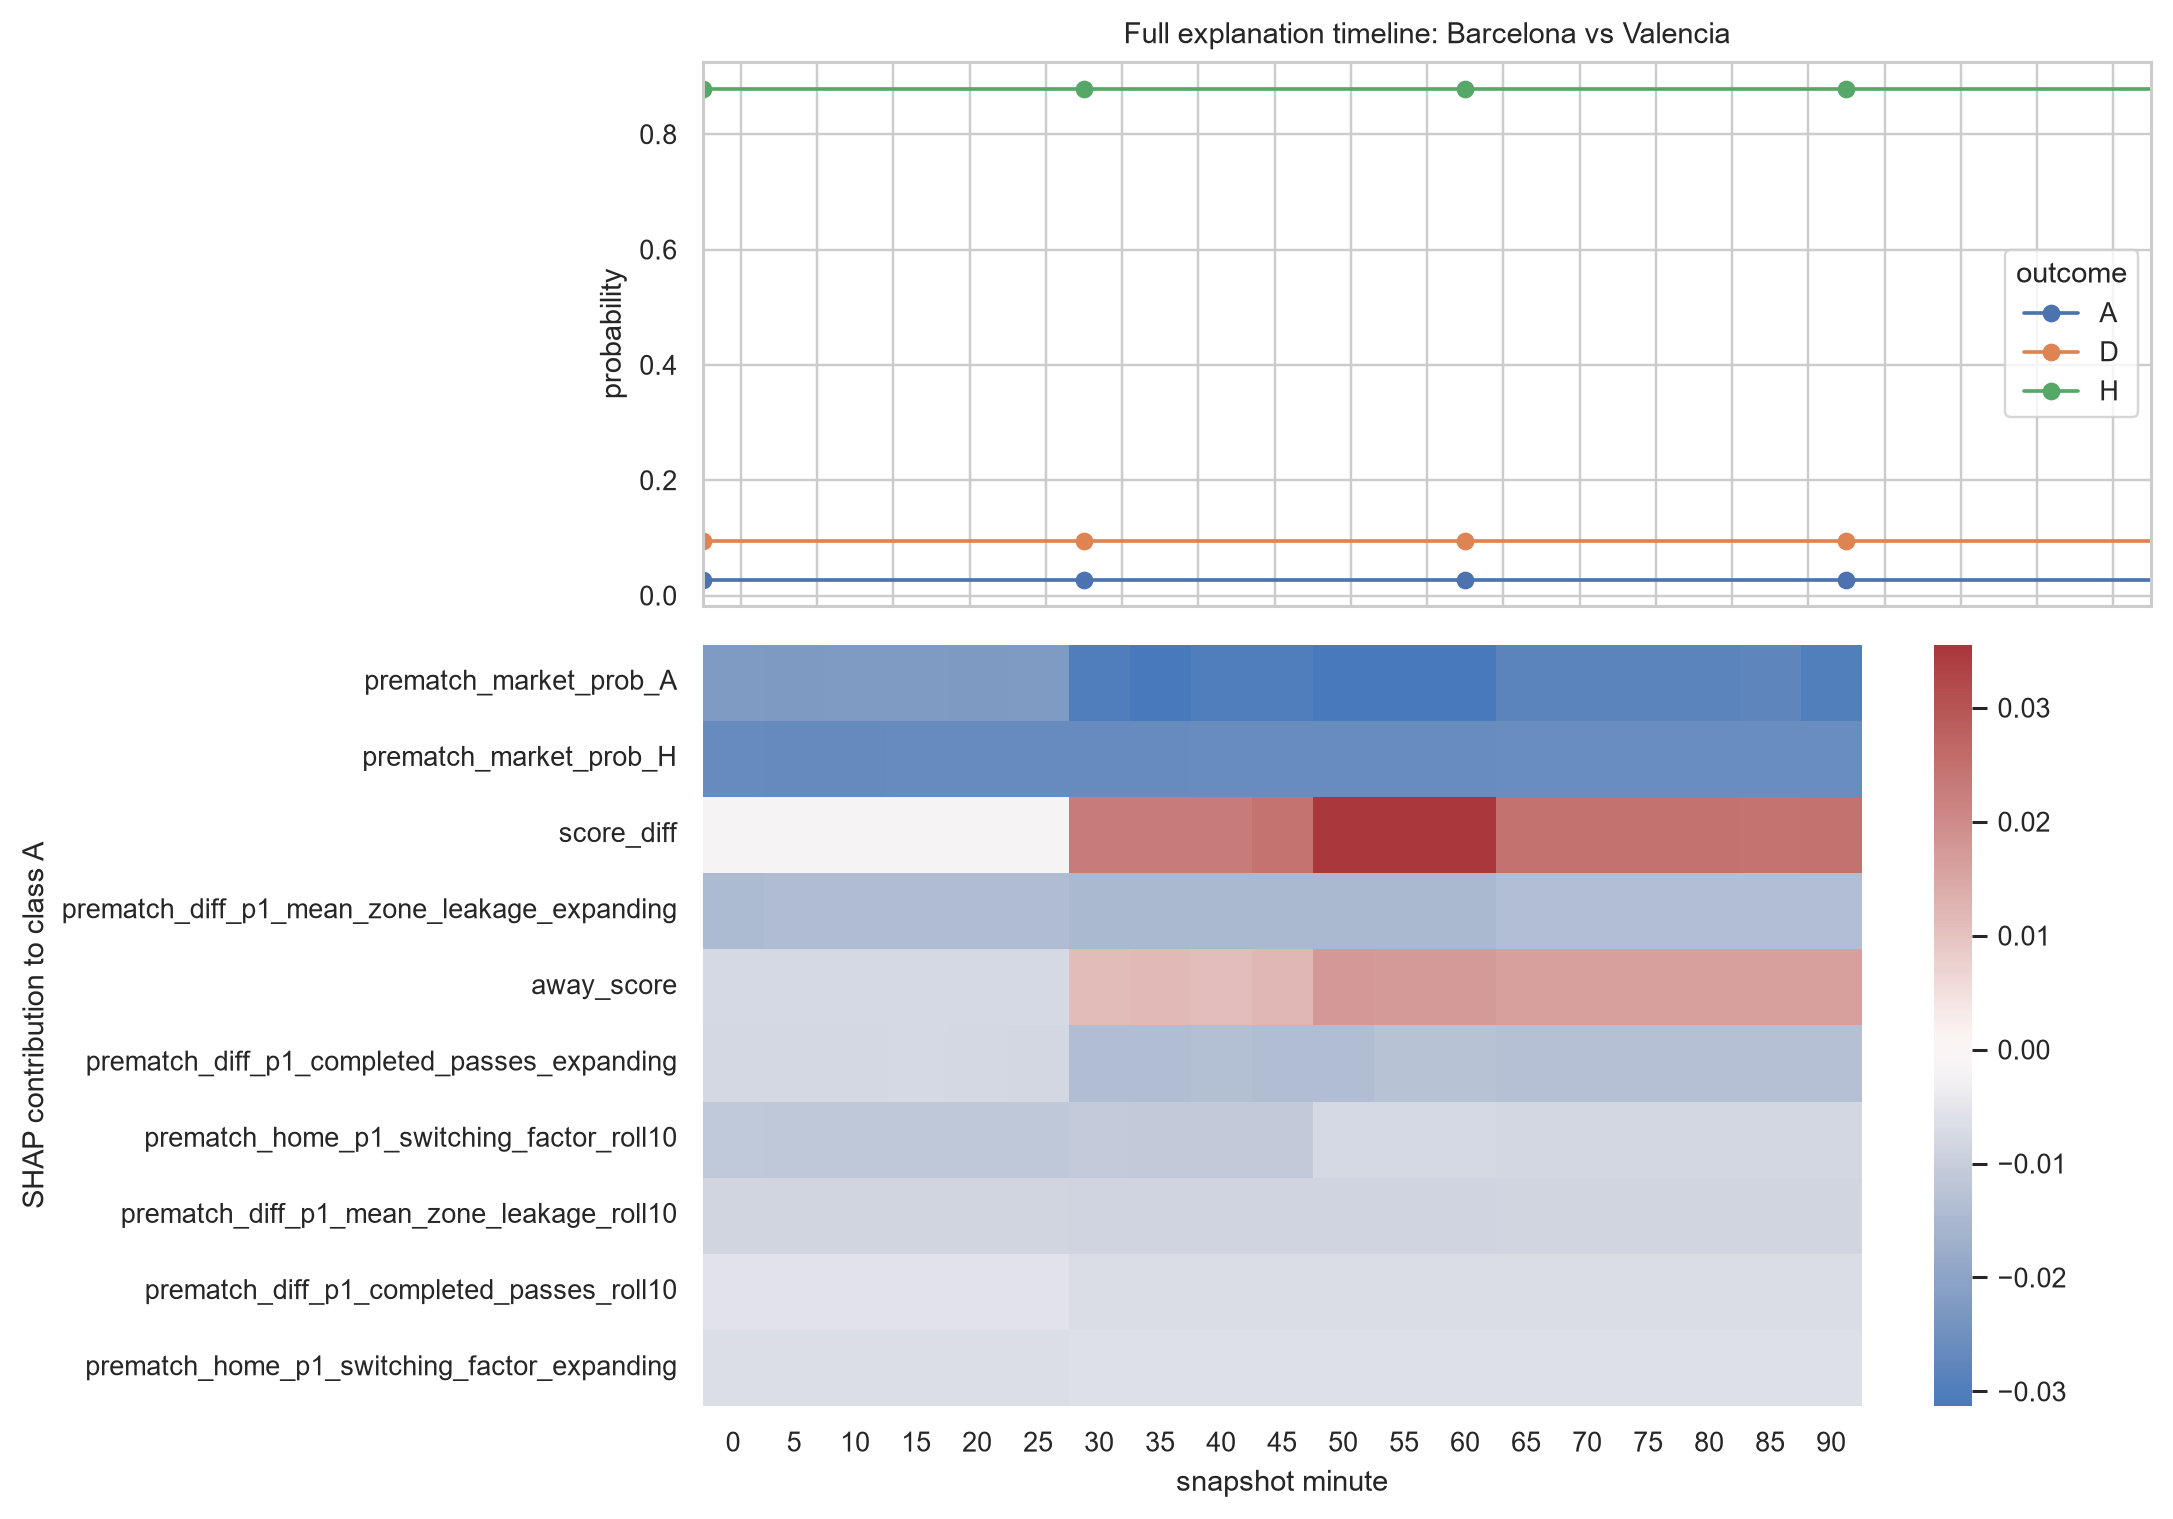
\includegraphics[width=.92\textwidth]{explainability/full_match_explanation_timeline.png}
\caption{One full 19-snapshot SHAP timeline. The selected Barcelona--Valencia failure remains overconfident in H while score state and class-A contributions evolve.}
\end{figure}

\subsection*{8C. Imbalance \& Resampling Discussion}

Development outcomes contain 183 H, 105 A, and 92 D matches. Training-only vanilla, class weighting, SMOTE, Borderline-SMOTE, and ADASYN are compared for a standardized logistic baseline. Vanilla has the best validation RPS (0.277); every synthetic variant worsens it. For snapshots, only class weighting is allowed: RF improves slightly from 0.149 to 0.146 validation RPS. No synthetic snapshot is created because it would mix physically incompatible match states and inflate within-match dependence.

\begin{figure}[H]
\centering
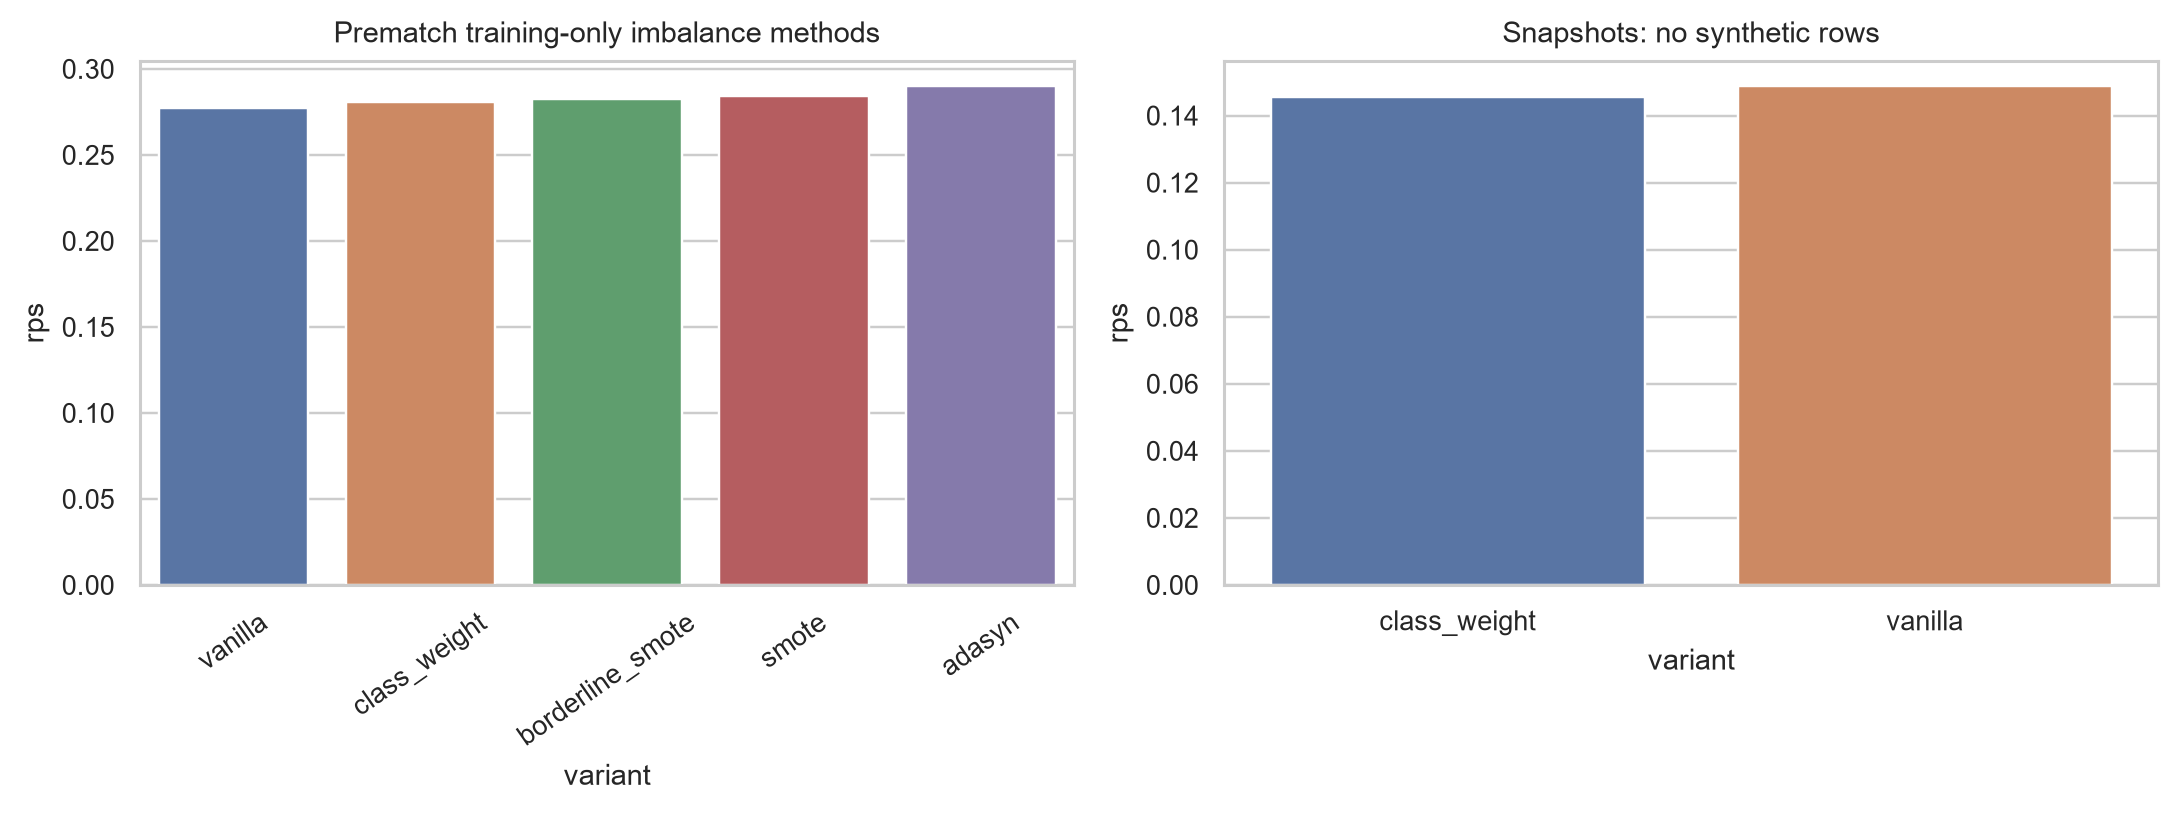
\includegraphics[width=.72\textwidth]{models/imbalance_comparison.png}
\caption{Imbalance experiments. Synthetic prematch sampling is training-only; snapshot counts remain genuine.}
\end{figure}

\subsection*{8D. Compute \& Scaling Analysis}

Instrumented development fitting totals 103 seconds and final refitting 77 seconds on the supplied machine, with observed process RSS below 560 MB. Exact kernel ridge forms an $n\times n$ Gram matrix: measured elements grow from 2,500 at $n=50$ to 35,721 at $n=189$. Nystroem uses $nm$ elements (14,175 at $n=189,m=75$). Times are similar at this small scale, but exact storage is $O(n^2)$ and becomes the limiting design at multi-season scale. P1 reconstruction is separately expensive (about 8.4 minutes for 414 matches) because boundary-aware possession segmentation and eigensystems are computed per fixture; saved matrices avoid repeated cost.

\begin{figure}[H]
\centering
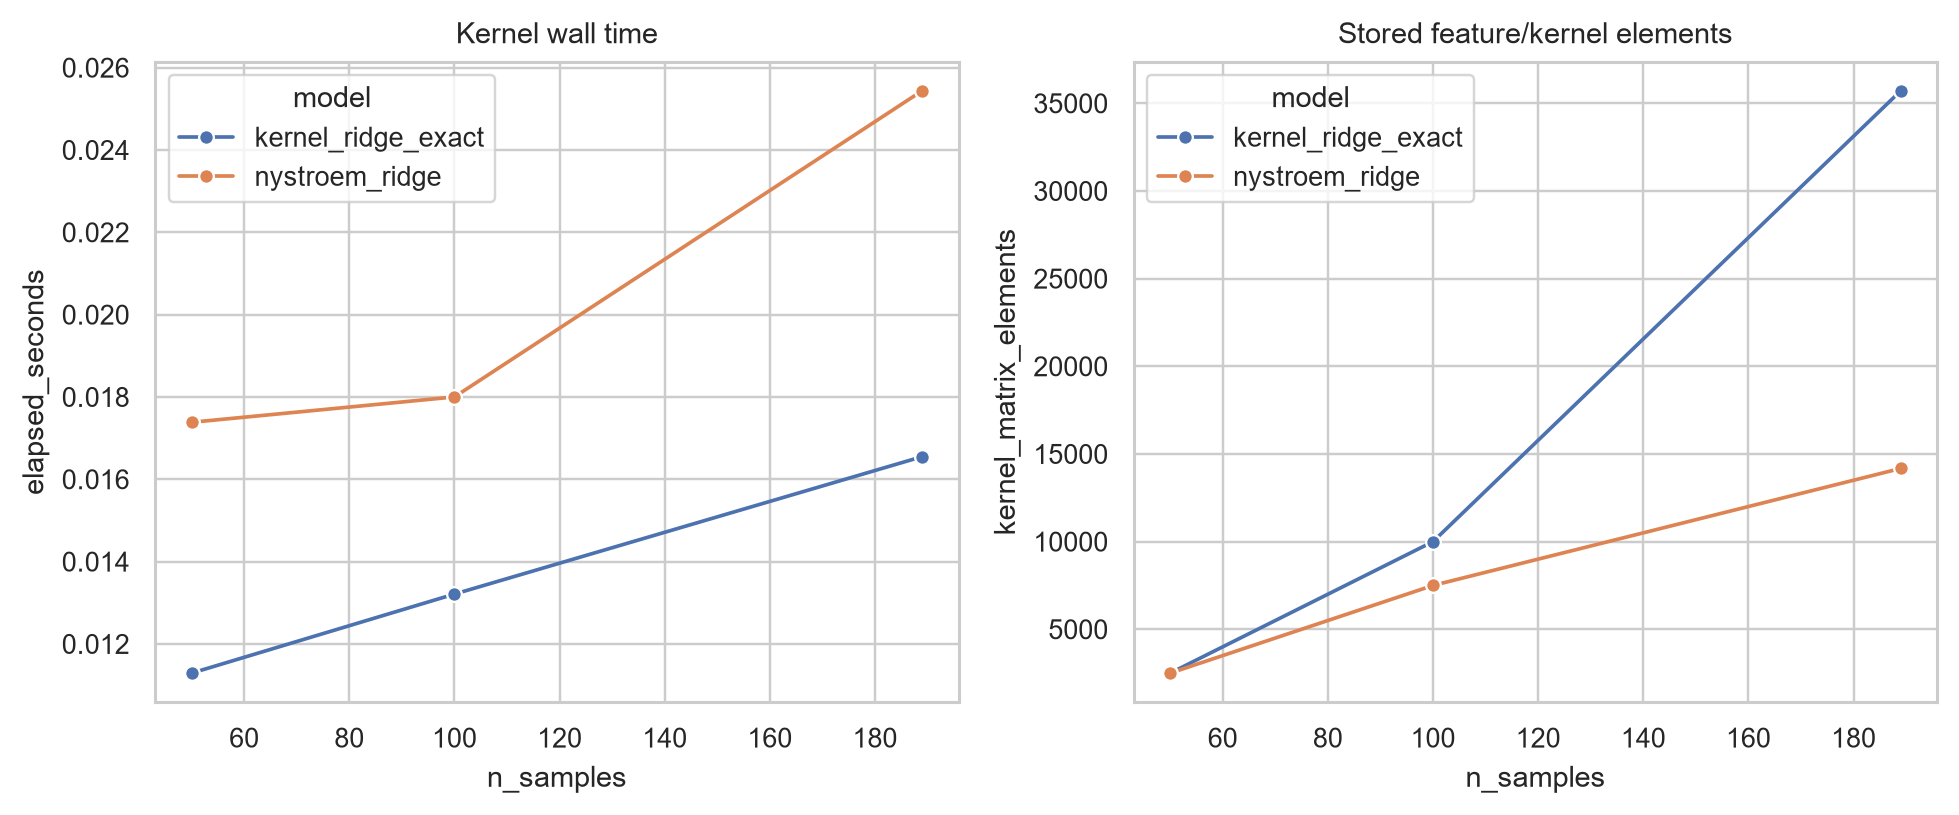
\includegraphics[width=.7\textwidth]{models/kernel_scaling.png}
\caption{Exact versus Nystroem kernel scaling. Small-$n$ wall time hides the quadratic exact representation.}
\end{figure}

\subsection*{8E. Theory vs. Reality}

Five gaps matter. First, P1's formulas transfer, but its Opta/2018--19 numerical claims do not. Second, FIGS' additive inductive bias is interpretable, yet scratch FIGS is not uniformly more accurate than ensembles; late in-play performance is its strongest use. Third, market information dominates development and many SHAP explanations, so a ``combined'' model can overfit hundreds of weak histories. Fourth, calibration improves reliability selectively and may worsen RPS under small holdouts. Fifth, the only fresh open-data season is a 34-match Barcelona-centred subset, creating both label imbalance (17 H, 12 A, 5 D) and severe fixture-selection shift. None can be repaired honestly by stronger claims.

\section{Conclusion \& Limitations}

The project delivers three leakage-safe tasks, a normalized integration layer, exact snapshots, tested P1 metrics, independent scratch FIGS, full required baselines, held-out calibration, imbalance/ablation/SHAP/error/compute analyses, and a one-shot final evaluation. The most defensible result is not that ML beats the market: RF/Platt's apparent 0.012 RPS improvement is uncertain. Live events do add value late, and compact FIGS becomes competitive in that regime.

Limitations are the 34-match selected final cohort, incomplete 2016/17 histories, one development season, small calibration blocks, absent 360, source-specific event semantics, and observational P1 associations. Historical Git metadata and TA sign-off were absent from the supplied directory and cannot be manufactured. Future work should acquire full later seasons under licence, use nested multi-season temporal validation, estimate calibration with more independent matches, and retest network features under stable competition coverage.

\clearpage
\appendix
\section{Hand Derivation of the P2 Core Update}

Let the current model be $F(x)=\sum_{k=1}^{K}T_k(x)$. For a candidate leaf $S$ in tree $k$, define the target excluding that tree:
\[
r_i^{(-k)}=y_i-\sum_{\ell\ne k}T_\ell(x_i).
\]
Tree $k$ is constant on an unsplit leaf, so excluding its current constant does not change which split maximizes squared-error decrease. If feature/threshold $(j,c)$ partitions $S$ into $L$ and $R$, optimal child constants are obtained by differentiation:
\[
v_L^*=\arg\min_v\sum_{i\in L}(r_i^{(-k)}-v)^2=\bar r_L^{(-k)},\qquad
v_R^*=\bar r_R^{(-k)}.
\]
The candidate gain is
\[
\Delta(S,j,c)=\sum_{i\in S}(r_i^{(-k)}-\bar r_S)^2-
\sum_{i\in L}(r_i^{(-k)}-\bar r_L)^2-
\sum_{i\in R}(r_i^{(-k)}-\bar r_R)^2.
\]
At each step FIGS evaluates this quantity for every current leaf and for a fresh root with $T_{K+1}=0$, accepts the global maximum, refreshes residuals for all trees, and stops at the total split budget. Hence an earlier tree can be revisited after another begins, unlike stagewise boosting. The supplement's backfitting fixes structure and alternates the same conditional means across trees, so squared training error cannot increase.

For multiclass reference behavior, $y_i$ is a one-hot vector and the same derivation applies componentwise with vector means. Summed scores $z_i=\sum_kT_k(x_i)$ become probabilities through $p_{ic}=\exp z_{ic}/\sum_d\exp z_{id}$. This is the behavior validated against \texttt{imodels}; it is explicitly different from the paper prose's Gini shorthand. With $d$ features, $n$ samples, and $m$ accepted splits, the supplement derives worst-case $O(dm^2n^2)$ growth versus CART's $O(dmn^2)$ because all candidate leaves are revisited.

\section{Reproducibility Appendix}

\textbf{Environment.} Python 3.13.7; NumPy 2.5.2; pandas 3.0.5; SciPy 1.18.0; scikit-learn 1.9.0; XGBoost 3.4.1; LightGBM 4.7.0; SHAP 0.52.0; pyarrow 21.0.0. Exact pins appear in \texttt{requirements.txt}, \texttt{environment.yml}, and \texttt{pyproject.toml}. Random seed is 42.

\textbf{Commands.}
\begin{verbatim}
conda env create -f environment.yml
conda activate football-ml
python -m pip install -e .
python -m pytest
football-ml-reproduce --stage data
football-ml-reproduce --stage features
football-ml-reproduce --stage development
football-ml-reproduce --stage artifacts
python scripts/build_report.py
\end{verbatim}
The final evaluator is intentionally absent from ordinary reproduction because its completed marker now prevents a second opening. Sixteen tests pass. Data, feature, split, and final-lock SHA-256 hashes are stored beside artifacts.

\textbf{Git and sign-off.} The received directory was not a Git repository; \texttt{git status} and \texttt{git log --oneline --all} failed before implementation. No historical commits were fabricated. No TA approval record was supplied. Genuine P1/P2 sign-off must be attached by the student. These two external requirements remain openly unresolved.

\begin{thebibliography}{9}
\bibitem{statsbomb} StatsBomb. \emph{StatsBomb Open Data}. GitHub repository, accessed 2026. \url{https://github.com/statsbomb/open-data}.
\bibitem{footballdata} Football-Data. \emph{Historical football results and betting odds: Spain Primera Division}. Accessed 2026. \url{https://www.football-data.co.uk/spainm.php}.
\bibitem{novillo2024} A. Novillo, B. Gong, J. H. Mart\'inez, R. Resta, R. L\'opez del Campo, and J. M. Buld\'u. ``A multilayer network framework for soccer analysis.'' \emph{Chaos, Solitons \& Fractals}, 178:114355, 2024. doi:10.1016/j.chaos.2023.114355.
\bibitem{tan2025} Y. S. Tan, C. Singh, K. Nasseri, A. Agarwal, et al. ``Fast Interpretable Greedy-Tree Sums.'' \emph{Proceedings of the National Academy of Sciences}, 2025. doi:10.1073/pnas.2310151122.
\bibitem{xgboost} T. Chen and C. Guestrin. ``XGBoost: A Scalable Tree Boosting System.'' \emph{KDD}, 2016.
\bibitem{lightgbm} G. Ke et al. ``LightGBM: A Highly Efficient Gradient Boosting Decision Tree.'' \emph{NeurIPS}, 2017.
\bibitem{shap} S. Lundberg and S.-I. Lee. ``A Unified Approach to Interpreting Model Predictions.'' \emph{NeurIPS}, 2017.
\bibitem{sklearn} F. Pedregosa et al. ``Scikit-learn: Machine Learning in Python.'' \emph{JMLR}, 12:2825--2830, 2011.
\end{thebibliography}

\end{document}
